% Options for packages loaded elsewhere
\PassOptionsToPackage{unicode}{hyperref}
\PassOptionsToPackage{hyphens}{url}
%
\documentclass[
]{book}
\usepackage{amsmath,amssymb}
\usepackage{iftex}
\ifPDFTeX
  \usepackage[T1]{fontenc}
  \usepackage[utf8]{inputenc}
  \usepackage{textcomp} % provide euro and other symbols
\else % if luatex or xetex
  \usepackage{unicode-math} % this also loads fontspec
  \defaultfontfeatures{Scale=MatchLowercase}
  \defaultfontfeatures[\rmfamily]{Ligatures=TeX,Scale=1}
\fi
\usepackage{lmodern}
\ifPDFTeX\else
  % xetex/luatex font selection
\fi
% Use upquote if available, for straight quotes in verbatim environments
\IfFileExists{upquote.sty}{\usepackage{upquote}}{}
\IfFileExists{microtype.sty}{% use microtype if available
  \usepackage[]{microtype}
  \UseMicrotypeSet[protrusion]{basicmath} % disable protrusion for tt fonts
}{}
\makeatletter
\@ifundefined{KOMAClassName}{% if non-KOMA class
  \IfFileExists{parskip.sty}{%
    \usepackage{parskip}
  }{% else
    \setlength{\parindent}{0pt}
    \setlength{\parskip}{6pt plus 2pt minus 1pt}}
}{% if KOMA class
  \KOMAoptions{parskip=half}}
\makeatother
\usepackage{xcolor}
\usepackage{color}
\usepackage{fancyvrb}
\newcommand{\VerbBar}{|}
\newcommand{\VERB}{\Verb[commandchars=\\\{\}]}
\DefineVerbatimEnvironment{Highlighting}{Verbatim}{commandchars=\\\{\}}
% Add ',fontsize=\small' for more characters per line
\usepackage{framed}
\definecolor{shadecolor}{RGB}{248,248,248}
\newenvironment{Shaded}{\begin{snugshade}}{\end{snugshade}}
\newcommand{\AlertTok}[1]{\textcolor[rgb]{0.94,0.16,0.16}{#1}}
\newcommand{\AnnotationTok}[1]{\textcolor[rgb]{0.56,0.35,0.01}{\textbf{\textit{#1}}}}
\newcommand{\AttributeTok}[1]{\textcolor[rgb]{0.13,0.29,0.53}{#1}}
\newcommand{\BaseNTok}[1]{\textcolor[rgb]{0.00,0.00,0.81}{#1}}
\newcommand{\BuiltInTok}[1]{#1}
\newcommand{\CharTok}[1]{\textcolor[rgb]{0.31,0.60,0.02}{#1}}
\newcommand{\CommentTok}[1]{\textcolor[rgb]{0.56,0.35,0.01}{\textit{#1}}}
\newcommand{\CommentVarTok}[1]{\textcolor[rgb]{0.56,0.35,0.01}{\textbf{\textit{#1}}}}
\newcommand{\ConstantTok}[1]{\textcolor[rgb]{0.56,0.35,0.01}{#1}}
\newcommand{\ControlFlowTok}[1]{\textcolor[rgb]{0.13,0.29,0.53}{\textbf{#1}}}
\newcommand{\DataTypeTok}[1]{\textcolor[rgb]{0.13,0.29,0.53}{#1}}
\newcommand{\DecValTok}[1]{\textcolor[rgb]{0.00,0.00,0.81}{#1}}
\newcommand{\DocumentationTok}[1]{\textcolor[rgb]{0.56,0.35,0.01}{\textbf{\textit{#1}}}}
\newcommand{\ErrorTok}[1]{\textcolor[rgb]{0.64,0.00,0.00}{\textbf{#1}}}
\newcommand{\ExtensionTok}[1]{#1}
\newcommand{\FloatTok}[1]{\textcolor[rgb]{0.00,0.00,0.81}{#1}}
\newcommand{\FunctionTok}[1]{\textcolor[rgb]{0.13,0.29,0.53}{\textbf{#1}}}
\newcommand{\ImportTok}[1]{#1}
\newcommand{\InformationTok}[1]{\textcolor[rgb]{0.56,0.35,0.01}{\textbf{\textit{#1}}}}
\newcommand{\KeywordTok}[1]{\textcolor[rgb]{0.13,0.29,0.53}{\textbf{#1}}}
\newcommand{\NormalTok}[1]{#1}
\newcommand{\OperatorTok}[1]{\textcolor[rgb]{0.81,0.36,0.00}{\textbf{#1}}}
\newcommand{\OtherTok}[1]{\textcolor[rgb]{0.56,0.35,0.01}{#1}}
\newcommand{\PreprocessorTok}[1]{\textcolor[rgb]{0.56,0.35,0.01}{\textit{#1}}}
\newcommand{\RegionMarkerTok}[1]{#1}
\newcommand{\SpecialCharTok}[1]{\textcolor[rgb]{0.81,0.36,0.00}{\textbf{#1}}}
\newcommand{\SpecialStringTok}[1]{\textcolor[rgb]{0.31,0.60,0.02}{#1}}
\newcommand{\StringTok}[1]{\textcolor[rgb]{0.31,0.60,0.02}{#1}}
\newcommand{\VariableTok}[1]{\textcolor[rgb]{0.00,0.00,0.00}{#1}}
\newcommand{\VerbatimStringTok}[1]{\textcolor[rgb]{0.31,0.60,0.02}{#1}}
\newcommand{\WarningTok}[1]{\textcolor[rgb]{0.56,0.35,0.01}{\textbf{\textit{#1}}}}
\usepackage{longtable,booktabs,array}
\usepackage{calc} % for calculating minipage widths
% Correct order of tables after \paragraph or \subparagraph
\usepackage{etoolbox}
\makeatletter
\patchcmd\longtable{\par}{\if@noskipsec\mbox{}\fi\par}{}{}
\makeatother
% Allow footnotes in longtable head/foot
\IfFileExists{footnotehyper.sty}{\usepackage{footnotehyper}}{\usepackage{footnote}}
\makesavenoteenv{longtable}
\usepackage{graphicx}
\makeatletter
\def\maxwidth{\ifdim\Gin@nat@width>\linewidth\linewidth\else\Gin@nat@width\fi}
\def\maxheight{\ifdim\Gin@nat@height>\textheight\textheight\else\Gin@nat@height\fi}
\makeatother
% Scale images if necessary, so that they will not overflow the page
% margins by default, and it is still possible to overwrite the defaults
% using explicit options in \includegraphics[width, height, ...]{}
\setkeys{Gin}{width=\maxwidth,height=\maxheight,keepaspectratio}
% Set default figure placement to htbp
\makeatletter
\def\fps@figure{htbp}
\makeatother
\setlength{\emergencystretch}{3em} % prevent overfull lines
\providecommand{\tightlist}{%
  \setlength{\itemsep}{0pt}\setlength{\parskip}{0pt}}
\setcounter{secnumdepth}{5}
\usepackage{booktabs}
\ifLuaTeX
  \usepackage{selnolig}  % disable illegal ligatures
\fi
\usepackage[]{natbib}
\bibliographystyle{plainnat}
\usepackage{bookmark}
\IfFileExists{xurl.sty}{\usepackage{xurl}}{} % add URL line breaks if available
\urlstyle{same}
\hypersetup{
  pdftitle={FishSimGTG: Population dynamics simulation framework},
  hidelinks,
  pdfcreator={LaTeX via pandoc}}

\title{FishSimGTG: Population dynamics simulation framework}
\author{\begin{center}
William J Harford  
\newline
Version 1.0.4
\newline
2024-08-23
\end{center}}
\date{}

\begin{document}
\maketitle

{
\setcounter{tocdepth}{1}
\tableofcontents
}
\chapter{What is FishSimGTG?}\label{what-is-fishsimgtg}

\textbf{FishSimGTG} is an R package that conducts numerical modeling of fish populations, including management strategy evaluation (MSE) and is an age-structured model that represents multiple concurrent cohorts using the growth-type-group methodology \citep{walters_fisheries_2004}. This framework is typically used to quantify trade-offs among competing management strategies or management options in terms of expected achievement of fishery management objectives. These trade-offs emerge from modeling results that are obtained from analysis methods like management strategy evaluation (MSE) or population dynamics projection. Calculation of trade-offs can play a meaningful role in supporting the development fishery management plans and fishery rule making. Simulations are implemented in the R statistical computing environment \citep{r_core_team_r_2022}. This framework is not a `black box' software, and thus, it is intended to be customized to address specific questions related to fishery management. This summary describes the base configuration of the population dynamics equations used in the simulation framework. Please be aware that this configuration can be tailored to specific applications.

\section{Installation and required packages}\label{installation-and-required-packages}

\textbf{FishSimGTG} is coded in R \citep{r_core_team_r_2022} and requires some basic packages that can be installed as follows:

\begin{enumerate}
\def\labelenumi{\arabic{enumi}.}
\item
  \textbf{Install R}:

  \begin{itemize}
  \tightlist
  \item
    Go to the \href{https://cran.r-project.org/}{CRAN website}.
  \item
    Download and install the appropriate version of R for your operating system (Windows, macOS, or Linux).
  \end{itemize}
\item
  \textbf{Install RStudio}:

  \begin{itemize}
  \tightlist
  \item
    Go to the \href{https://www.rstudio.com/products/rstudio/download/}{RStudio website}.
  \item
    Download and install RStudio Desktop (free version).
  \end{itemize}
\item
  \textbf{Installing Required Packages}:
\end{enumerate}

The user can install the necessary packages to run the simulation and visualize the outputs by using the following R commands:

\begin{Shaded}
\begin{Highlighting}[]
\FunctionTok{install.packages}\NormalTok{(}\StringTok{"devtools"}\NormalTok{)}
\NormalTok{devtools}\SpecialCharTok{::}\FunctionTok{install\_github}\NormalTok{(}\StringTok{"natureanalytics{-}ca/fishSimGTG@v1.0.6"}\NormalTok{)}
\NormalTok{devtools}\SpecialCharTok{::}\FunctionTok{install\_github}\NormalTok{(}\StringTok{"natureanalytics{-}ca/fishSimTools@v0.0.0.9"}\NormalTok{)}
\FunctionTok{install.packages}\NormalTok{(}\StringTok{"here"}\NormalTok{)}
\end{Highlighting}
\end{Shaded}

\begin{enumerate}
\def\labelenumi{\arabic{enumi}.}
\setcounter{enumi}{3}
\tightlist
\item
  \textbf{Load the Required Packages}:
\end{enumerate}

\begin{Shaded}
\begin{Highlighting}[]
\FunctionTok{library}\NormalTok{(devtools)}
\FunctionTok{library}\NormalTok{(fishSimGTG)}
\FunctionTok{library}\NormalTok{(fishSimTools)}
\FunctionTok{library}\NormalTok{(here)}
\end{Highlighting}
\end{Shaded}

The core packages required to run the simulation are \texttt{fishSimGTG} and \texttt{fishSimTools}. The \texttt{devtools} package is necessary because it allows us to install these core packages directly from GitHub, ensuring we have the latest versions and updates. The \texttt{here} package is essential for simplifying file referencing in project-oriented workflows, making it easier to manage and navigate project files consistently.

\section{How to use FishSimGTG?}\label{how-to-use-fishsimgtg}

The \textbf{FishSimGTG} package can be used to construct an operating model (OM) that simulates population and fishery dynamics, including data collection and the application of user-customized management procedures. The OM consists of several S4-type objects, such as the \texttt{LifeHistory} object, \texttt{Fishery} object, and \texttt{TimeArea} object, etc. These objects store parameters and information in slots, which users can access using the \texttt{@} symbol.

The simplest way to start building the OM is to create a new object using the R function \texttt{new()} and populate it with the required input information and parameters. The next chapter provides a full description of the S4 object components and instructions on how to populate each object to create the OM.

\chapter{How to Populate the Operating Model (OM)}\label{OM-pop}

The OM is comprised of six S4 objects:

\begin{itemize}
\tightlist
\item
  Life history object (\texttt{LifeHistoryObj})
\item
  Fishery object (\texttt{HistFisheryObj})
\item
  Time-area object (\texttt{TimeAreaObj})
\item
  Stochastic object (\texttt{StochasticObj})
  Separate section
\item
  Projection object (\texttt{ProFisheryObj})
\item
  Strategy object (\texttt{StrategyObj})
\end{itemize}

Each of these S4 objects contains a specific number of slots, which can be accessed using the \texttt{slotNames()} function. These slots are populated within R. The first step, before populating the slots of each object, is to create a new object using the \texttt{new()} function.

\section{Life history object}\label{life-history-object}

The \texttt{LifeHistoryObj} is an S4 object of the class \texttt{LifeHistory} that holds the description of a life history.
To create a new object of class \texttt{LifeHistory}, use the \texttt{new()} function, as follows:

\begin{Shaded}
\begin{Highlighting}[]
\NormalTok{LifeHistoryObj }\OtherTok{\textless{}{-}} \FunctionTok{new}\NormalTok{(}\StringTok{"LifeHistory"}\NormalTok{)}
\end{Highlighting}
\end{Shaded}

The user can see the elements or slots of the \texttt{LifeHistoryObject} using the \texttt{slotNames()} function.

\begin{Shaded}
\begin{Highlighting}[]
\FunctionTok{slotNames}\NormalTok{(LifeHistoryObj)}
\end{Highlighting}
\end{Shaded}

\begin{verbatim}
##  [1] "title"            "speciesName"      "shortDescription" "L_type"          
##  [5] "L_units"          "Walpha_units"     "Linf"             "K"               
##  [9] "t0"               "L50"              "L95delta"         "M"               
## [13] "MK"               "LW_A"             "LW_B"             "Tmax"            
## [17] "Steep"            "R0"               "recSD"            "recRho"          
## [21] "isHermaph"        "H50"              "H95delta"
\end{verbatim}

The user can access the help file for classes by using \texttt{?} symbol

\begin{Shaded}
\begin{Highlighting}[]
\NormalTok{?}\StringTok{\textasciigrave{}}\AttributeTok{LifeHistory{-}class}\StringTok{\textasciigrave{}}  
\end{Highlighting}
\end{Shaded}

In the help file, the user will find a description of the \texttt{LifeHistoryObject} and the elements or slots it contains. To populate the rest of the slots of the \texttt{LifeHistoryObject}, the user should start by defining a useful title (\texttt{title}), followed by the scientific name of the species (\texttt{speciesName}). If desired, the user can add a short description (\texttt{shortDescription}) of the object.

\begin{Shaded}
\begin{Highlighting}[]
\NormalTok{LifeHistoryObj}\SpecialCharTok{@}\NormalTok{title}\OtherTok{\textless{}{-}}\StringTok{"Kole"}
\NormalTok{LifeHistoryObj}\SpecialCharTok{@}\NormalTok{speciesName}\OtherTok{\textless{}{-}}\StringTok{"Ctenochaetus strigosus"}
\NormalTok{LifeHistoryObj}\SpecialCharTok{@}\NormalTok{shortDescription}\OtherTok{\textless{}{-}}\StringTok{"stock name/location"}
\end{Highlighting}
\end{Shaded}

Then, the user can proceed to populate the rest of the slots as follows:

\begin{Shaded}
\begin{Highlighting}[]
\NormalTok{LifeHistoryObj}\SpecialCharTok{@}\NormalTok{Linf}\OtherTok{\textless{}{-}}\FloatTok{17.7}
\NormalTok{LifeHistoryObj}\SpecialCharTok{@}\NormalTok{K}\OtherTok{\textless{}{-}}\FloatTok{0.423}
\NormalTok{LifeHistoryObj}\SpecialCharTok{@}\NormalTok{t0}\OtherTok{\textless{}{-}} \SpecialCharTok{{-}}\FloatTok{0.51}
\NormalTok{LifeHistoryObj}\SpecialCharTok{@}\NormalTok{L50}\OtherTok{\textless{}{-}}\FloatTok{8.4}
\NormalTok{LifeHistoryObj}\SpecialCharTok{@}\NormalTok{L95delta}\OtherTok{\textless{}{-}}\FloatTok{1.26}
\NormalTok{LifeHistoryObj}\SpecialCharTok{@}\NormalTok{M}\OtherTok{\textless{}{-}}\FloatTok{0.08}
\NormalTok{LifeHistoryObj}\SpecialCharTok{@}\NormalTok{L\_type}\OtherTok{\textless{}{-}}\StringTok{"FL"}
\NormalTok{LifeHistoryObj}\SpecialCharTok{@}\NormalTok{L\_units}\OtherTok{\textless{}{-}}\StringTok{"cm"}
\NormalTok{LifeHistoryObj}\SpecialCharTok{@}\NormalTok{LW\_A}\OtherTok{\textless{}{-}}\FloatTok{0.046}
\NormalTok{LifeHistoryObj}\SpecialCharTok{@}\NormalTok{LW\_B}\OtherTok{\textless{}{-}}\FloatTok{2.85}
\NormalTok{LifeHistoryObj}\SpecialCharTok{@}\NormalTok{Steep}\OtherTok{\textless{}{-}}\FloatTok{0.54}
\NormalTok{LifeHistoryObj}\SpecialCharTok{@}\NormalTok{recSD}\OtherTok{\textless{}{-}}\DecValTok{0}
\NormalTok{LifeHistoryObj}\SpecialCharTok{@}\NormalTok{recRho}\OtherTok{\textless{}{-}}\DecValTok{0}
\NormalTok{LifeHistoryObj}\SpecialCharTok{@}\NormalTok{isHermaph}\OtherTok{\textless{}{-}}\ConstantTok{FALSE}
\NormalTok{LifeHistoryObj}\SpecialCharTok{@}\NormalTok{R0}\OtherTok{\textless{}{-}}\DecValTok{10000}
\end{Highlighting}
\end{Shaded}

Growth is modeled in the \textbf{FishSimGTG} package using a von Bertalanffy growth curve, where \texttt{Linf} represents the asymptotic average length, \texttt{K} the Brody growth rate coefficient (with units in yr\(^{-1}\)), and \texttt{t0} represents the time or age when the average length was zero.

Maturity parameters are represented by the \texttt{L50} and \texttt{L95delta} parameters, assuming that maturity is size-dependent and follows a logistic model. The \texttt{L50} is the length at 50\% maturity, and the \texttt{L95delta} is the length increment between L50 and the length at 95\% maturity. \texttt{L95delta} must be a value larger than 0.

\texttt{M}, represent the natural mortality rate per year.

\texttt{L\_type} represents the method of measuring length. e.g.~\texttt{"TL"} for total length or \texttt{"FL"} for fork length. Must be consistent for all length parameters (e.g., \texttt{Linf}, \texttt{L50}, \texttt{L95delta}). \texttt{L\_units}, are the units of measure (\texttt{"cm"} is expected). \texttt{L\_units} must be consistent for all length parameters (e.g., \texttt{Linf}, \texttt{L50}, \texttt{L95delta}).

\texttt{LW\_A} and \texttt{LW\_B} are the parameters of the allometric length-weight relationship. \texttt{Walpha\_units} (\textbf{ask bill/ in help says W\_units})represents the measurement units of weight and must be consistent with the \texttt{LW\_A} and \texttt{LW\_B} parameters.

Recruitment is modeled using a Beverton-Holt stock-recruitment relationship, parameterized in terms of steepness (\texttt{Steep}). Values for \texttt{Steep} range between 0.2 to 1. \texttt{R0} represents the initial number of unfished recruits (positive number). Recruitment process error is generated from a normal distribution with mean zero and standard deviation represented by \texttt{recSD}. Autocorrelation in recruitment deviations in log space are defined by \texttt{recRho}, producing 1-year lagged correlation. \texttt{recSD} and \texttt{recRho}, are non-negative real numbers.

The \textbf{FishSimGTG} package allows for modeling the population dynamics of gonochoristic and protogynous hermaphrodite species. The user will set \texttt{isHermaph} to \texttt{TRUE} when the species is a protogynous hermaphrodite and to \texttt{FALSE} when it is a gonochoristic species. If the species is a protogynous hermaphrodite, the user will need to define two additional parameters: \texttt{H50} and \texttt{H95delta}. \texttt{H50} represents the length at which 50\% of the population are male, and \texttt{H95delta} represents the length increment between \texttt{H50} and length at which 95\% of the population are male. \texttt{H95delta} must be a value larger than 0.

\texttt{MK} and \texttt{Tmax} are not esscencial input parameters. \texttt{MK} represents the M/K ratio (natural mortality divided by von Bertalanffy K coefficient) and \texttt{Tmax} the maximum observed age. (\textbf{ask bill}). \texttt{Tmax} must be equal to or greater than 2. When \texttt{Tmax} is not specified, the age to which 1\% the population survives in an unfished system is used to calculate \texttt{Tmax}.

\section{Fishery object}\label{fishery-object}

The \texttt{HistFisheryObj} is an S4 object of the class \texttt{Fishery} that holds the historical description of a fish stock, including vulnerability, retention, and discard information.
To create a new object of class \texttt{Fishery}, use the \texttt{new()} function, as follows:

\begin{Shaded}
\begin{Highlighting}[]
\NormalTok{HistFisheryObj}\OtherTok{\textless{}{-}}\FunctionTok{new}\NormalTok{(}\StringTok{"Fishery"}\NormalTok{)}
\end{Highlighting}
\end{Shaded}

The slot names of the \texttt{HistFisheryObj} can be seen using the \texttt{slotNames()} function.

\begin{Shaded}
\begin{Highlighting}[]
\FunctionTok{slotNames}\NormalTok{(HistFisheryObj)}
\end{Highlighting}
\end{Shaded}

\begin{verbatim}
## [1] "title"     "vulType"   "vulParams" "retType"   "retParams" "retMax"   
## [7] "Dmort"
\end{verbatim}

The user can access the help file using \texttt{?} symbol

\begin{Shaded}
\begin{Highlighting}[]
\NormalTok{?}\StringTok{\textasciigrave{}}\AttributeTok{Fishery{-}class}\StringTok{\textasciigrave{}}  
\end{Highlighting}
\end{Shaded}

In the help file, the user will find a description of the \texttt{HistFisheryObj} and the elements or slots it contains. To populate the slots, the user should start by defining a meaningful title (\texttt{title}), followed by specifying the selectivity/vulnerability, retention, and discard information.

\begin{Shaded}
\begin{Highlighting}[]
\NormalTok{HistFisheryObj}\SpecialCharTok{@}\NormalTok{title}\OtherTok{\textless{}{-}}\StringTok{"Test"}
\NormalTok{HistFisheryObj}\SpecialCharTok{@}\NormalTok{vulType}\OtherTok{\textless{}{-}}\StringTok{"logistic"}
\NormalTok{HistFisheryObj}\SpecialCharTok{@}\NormalTok{vulParams}\OtherTok{\textless{}{-}}\FunctionTok{c}\NormalTok{(}\FloatTok{10.2}\NormalTok{,}\FloatTok{0.1}\NormalTok{) }\CommentTok{\#Approx. knife edge}
\NormalTok{HistFisheryObj}\SpecialCharTok{@}\NormalTok{retType}\OtherTok{\textless{}{-}}\StringTok{"full"}
\NormalTok{HistFisheryObj}\SpecialCharTok{@}\NormalTok{retMax }\OtherTok{\textless{}{-}} \DecValTok{1}
\NormalTok{HistFisheryObj}\SpecialCharTok{@}\NormalTok{Dmort }\OtherTok{\textless{}{-}} \DecValTok{0}
\end{Highlighting}
\end{Shaded}

\subsection{Selectivity or vulnerability}\label{selectivity-or-vulnerability}

Selectivity or vulnerability is the probability of being selected or becoming vulnerable to the fishing gear. It can be defined as selectivity-at-age or selectivity-at-length. In the \textbf{FishSimGTG package}, selectivity is defined with respect to length, with a maximum value of 1 enforced.
\texttt{vulType} describes the type of selectivity/vulnerability function for the historical time period. The \textbf{FishSimGTG} package offers four options to model the selectivity shape: ``\textbf{logistic}'', ``\textbf{explog}'', ``\textbf{gillnetMasterNormal}'', and ``\textbf{gillnetMasterLognormal}''. The user can see a detailed description of the different selectivity functions by exploring the \texttt{?selWrapper} function.

Vulnerability types:

\begin{itemize}
\item
  ``\textbf{logistic}'' selectivity with two parameters (\texttt{vulParams}) represented by the length at 50\% of selectivity and the length increment between the length at 50\% of selectivity and the length at 95\% selectivity.
\item
  ``\textbf{explog}'' is an exponential logistic selectivity (dome-shaped) function, defined by three parameters (\texttt{vulParams}), represented as \texttt{c(p1,\ peak,\ and\ p3)}. To use the ``\textbf{explog}'' function, the user must first provide the ascending rate (p1), which should be within the range of 0.02 to 1. Next, the user needs to define the peak of the vulnerability function, which corresponds to the location of the peak of the dome-shaped selectivity curve or the length at which selectivity is highest. This peak is expressed as a fraction (p2), determining its position relative to the range of lengths. For example, if the length range is between 1 and 20 cm, and p2 is set to 0.5, the peak will be at 10 cm.
\end{itemize}

The peak can be calculated using the following equation:

\[
\text{peak} = \text{min}(\text{Length}) + p_2 \times (\text{max}(\text{Length}) - \text{min}(\text{Length}))
\]

p2 must be within the range of 0.01 to 0.9, with a reasonable starting value of 0.5. By adjusting p2, the user can shift the peak along the length range, from the minimum length to the maximum length.

p3 is the descending rate, which must be within the range of 0.001 to 0.5. A value of 0.001 provides a nearly asymptotic curve, while values above 0.2 produce a strongly dome-shaped function, where the p3 and p1 parameters interact strongly.

\textbf{Note: I suggest changing p2 by peak in the help file (i.e., c(p1, peak, p3) because what the user provides is the peak not p2 see Testing\_selectivity.R)}

\begin{itemize}
\tightlist
\item
  ``\textbf{gillnetMasterNormal}'' is a master curve for mesh selectivity with a vector of three parameter (\texttt{vulParams}), represented as \texttt{c(p1,\ p2,\ and\ p3)}. \texttt{p1} determines the peak or central point of the dome-shaped selectivity curve. It is referred to as the location parameter because it ``locates'' where the maximum selectivity occurs along the length vector. \texttt{p2} is the variance parameter that controls the spread or width of the selectivity curve. It is related to how quickly selectivity decreases from the peak. A smaller value of p2 results in a narrower peak, meaning selectivity drops off more sharply as you move away from the central point (p1), making the curve steeper. \texttt{p3} represents the mesh size and scales the length vector. By dividing the length by p3, the selectivity curve can be adjusted to reflect different mesh sizes used in the fishery.
\end{itemize}

When length vector/p3 equals p1, the selectivity function reaches its peak. For example, if p1 equals 2.5, the peak of selectivity will occur at the length when length/p3 equals 2.5.

(\textbf{ask Bill whether he agrees with this explanation})

\begin{itemize}
\tightlist
\item
  ``\textbf{gillnetMasterLognormal}'' is a master curve for mesh selectivity with a vector of three parameter (\texttt{vulParams}), represented as \texttt{c(p1,\ p2,\ and\ p3)}. These parameters are the same as those used in the ``\textbf{gillnetMasterNormal}'' selectivity function.
  The difference between ``\textbf{gillnetMasterNormal}'' and ``\textbf{gillnetMasterLognormal}'' lies in the logarithmic transformation applied in the ``\textbf{gillnetMasterLognormal}'' function, where length/p3 and p1 are log transformed.
\end{itemize}

The logarithmic transformation spreads out the curve, making it wider and less steep. This transformation smooths the effect of differences between length/p3 and p1, leading to a more gradual decrease in selectivity. Without using the logarithmic function, the selectivity curve becomes narrower and steeper, responding more sensitively to deviations from the peak.

(\textbf{ask Bill whether he agrees with this explanation})

\subsection{Retention}\label{retention}

Retention is the probability of being retained (kept by the fleet) and not discarded. It describes both the shape with respect to length and the maximum value, which can be less than 1. Fish that are selected by the fishing gear but not retained are discarded (discard mortality rate). The probability of being landed (\textbf{keep}), is calculated as Vulnerability × Retention. The user can see a detailed description of the different retention types by exploring the \texttt{?selWrapper} function.

There are three retention types (\texttt{retType}):

\begin{itemize}
\item
  ``\textbf{full}'' retention assumes that keep is equal to retention and that there is no discard mortality. There are no parameters (\texttt{retParams}) for ``full'' retention.
\item
  ``\textbf{logistic}'' retention has two parameters (\texttt{retParams}): the length at 50\% retention and the length increment to 95\% retention.
\item
  ``\textbf{slotLimit}'' retention includes two parameters (\texttt{retParams}): minimum length and maximum length, where catches occur between the minimum and maximum values.
\end{itemize}

\texttt{retMax} is a numeric value between 0 and 1 that defines the peak of the historical retention curve.

\subsection{Discard mortality rate}\label{discard-mortality-rate}

Discard mortality rate represents the fish that are selected but not retained, and are therefore subject to the discard mortality rate (\texttt{Dmort}). \texttt{Dmort} is the fraction of discards that are killed (e.g., 0.25 means 25\% are killed). This value must be between 0 and 1.

in Section \ref{lh-sel}, the user can explore various life history plots and different shapes of vulnerability, retention, keep, discard, and removal curves.

\section{Time area object}\label{time-area-object}

The \textbf{FishSimGTG} package allows the user to model migration between multiple areas. The \texttt{TimeAreaObj} object holds descriptions of time steps, growth-type groups (GTGs), and area parameters.

To create a new object of class \texttt{TimeArea}, use the \texttt{new()} function as follows:

\begin{Shaded}
\begin{Highlighting}[]
\NormalTok{TimeAreaObj}\OtherTok{\textless{}{-}}\FunctionTok{new}\NormalTok{(}\StringTok{"TimeArea"}\NormalTok{)}
\end{Highlighting}
\end{Shaded}

To populate the slots of the \texttt{TimeAreaObj} object, the user should start by defining a meaningful title (\texttt{title}). Similar to the other S4 objects, the slot names of the \texttt{TimeAreaObj} can be viewed using the \texttt{slotNames()} function, and the user can access the help file using the \texttt{?} symbol.

\begin{Shaded}
\begin{Highlighting}[]
\FunctionTok{slotNames}\NormalTok{(TimeAreaObj)}
\end{Highlighting}
\end{Shaded}

\begin{verbatim}
##  [1] "title"             "gtg"               "areas"            
##  [4] "recArea"           "move"              "iterations"       
##  [7] "historicalYears"   "historicalBio"     "historicalBioType"
## [10] "historicalEffort"
\end{verbatim}

\begin{Shaded}
\begin{Highlighting}[]
\CommentTok{\#getting help}
\NormalTok{?}\StringTok{\textasciigrave{}}\AttributeTok{TimeArea{-}class}\StringTok{\textasciigrave{}}  
\end{Highlighting}
\end{Shaded}

\begin{Shaded}
\begin{Highlighting}[]
\NormalTok{TimeAreaObj}\SpecialCharTok{@}\NormalTok{title }\OtherTok{=} \StringTok{"Test"}
\NormalTok{TimeAreaObj}\SpecialCharTok{@}\NormalTok{gtg }\OtherTok{=} \DecValTok{13}
\NormalTok{TimeAreaObj}\SpecialCharTok{@}\NormalTok{areas }\OtherTok{=} \DecValTok{2}
\NormalTok{TimeAreaObj}\SpecialCharTok{@}\NormalTok{recArea }\OtherTok{=} \FunctionTok{c}\NormalTok{(}\FloatTok{0.99}\NormalTok{, }\FloatTok{0.01}\NormalTok{)}
\NormalTok{TimeAreaObj}\SpecialCharTok{@}\NormalTok{iterations }\OtherTok{=} \DecValTok{100}
\NormalTok{TimeAreaObj}\SpecialCharTok{@}\NormalTok{historicalYears }\OtherTok{=} \DecValTok{10}
\NormalTok{TimeAreaObj}\SpecialCharTok{@}\NormalTok{historicalBio }\OtherTok{=} \FloatTok{0.5}
\NormalTok{TimeAreaObj}\SpecialCharTok{@}\NormalTok{historicalBioType }\OtherTok{=} \StringTok{"relB"}
\NormalTok{TimeAreaObj}\SpecialCharTok{@}\NormalTok{move }\OtherTok{\textless{}{-}} \FunctionTok{matrix}\NormalTok{(}\FunctionTok{c}\NormalTok{(}\DecValTok{1}\NormalTok{,}\DecValTok{0}\NormalTok{, }\DecValTok{0}\NormalTok{,}\DecValTok{1}\NormalTok{), }\AttributeTok{nrow=}\DecValTok{2}\NormalTok{, }\AttributeTok{ncol=}\DecValTok{2}\NormalTok{, }\AttributeTok{byrow=}\ConstantTok{FALSE}\NormalTok{)}
\NormalTok{TimeAreaObj}\SpecialCharTok{@}\NormalTok{historicalEffort}\OtherTok{\textless{}{-}}\FunctionTok{matrix}\NormalTok{(}\DecValTok{1}\SpecialCharTok{:}\DecValTok{1}\NormalTok{, }\AttributeTok{nrow =} \DecValTok{10}\NormalTok{, }\AttributeTok{ncol =} \DecValTok{2}\NormalTok{, }\AttributeTok{byrow =} \ConstantTok{FALSE}\NormalTok{)}
\end{Highlighting}
\end{Shaded}

The \textbf{FishSimGTG} package allows for accounting for individual variation in growth trajectories by dividing the population into growth-type groups (GTGs), so each age class is divided into a collection of smaller cohorts or GTGs. The \texttt{gtg} slot in \texttt{TimeAreaObj} represents the number of growth-type groups, with a default value of 13.(\textbf{ask Bill})

\texttt{areas} represents the number of areas in the model, and it must be greater than 1.

\texttt{recArea} is a vector of length \texttt{areas}. Each element of the vector represents the fraction of recruitment to each area, with the values summing to 1. In this example, 0.99 of the recruitment is assigned to area 1, and 0.01 to area 2, implying that the model is treated similarly to a single-area model.

\texttt{iterations} is the number of iterations to run.

\texttt{historicalYears} are the number of years to simulate historical dynamics.

\texttt{historicalBio} is a value grater than 0 and less than 1. The model assumes the population does not start in unfished conditions.

\texttt{historicalBioType}is a string, that represents the type of historical biomass state. The options are: ``relB'' (relative biomass) or ``SPR'' (Spawning Potential Ratio).

\texttt{move} is a matrix of migration rates of dimensions \texttt{areas} x \texttt{areas}.

\texttt{historicalEffort} is a matrix of nrows = \texttt{historicalYears} and ncols = \texttt{areas} that contains value multipiers of initial equilibrium fishing effort. (\textbf{ask bill}).

\subsection{Exploring the Parameterization of the Operating Model So Far}\label{lh-sel}

The \textbf{FishSimGTG} package includes several plotting functions that allow users to explore the simulated life history and the configuration of the fishery object.

\begin{itemize}
\tightlist
\item
  The life history schedules can be plotted using the \texttt{LHwrapper()} function. This function displays the plot in the console and also returns all the details of the life history. The user can access the help file for the \texttt{LHwrapper()} function by using the \texttt{?} symbol (\texttt{?LHwrapper}).
\end{itemize}

\begin{Shaded}
\begin{Highlighting}[]
\CommentTok{\#To simply display to the console}
\NormalTok{lhOut}\OtherTok{\textless{}{-}}\FunctionTok{LHwrapper}\NormalTok{(LifeHistoryObj, TimeAreaObj, }\AttributeTok{doPlot =} \ConstantTok{TRUE}\NormalTok{)}
\end{Highlighting}
\end{Shaded}

\begin{figure}
\centering
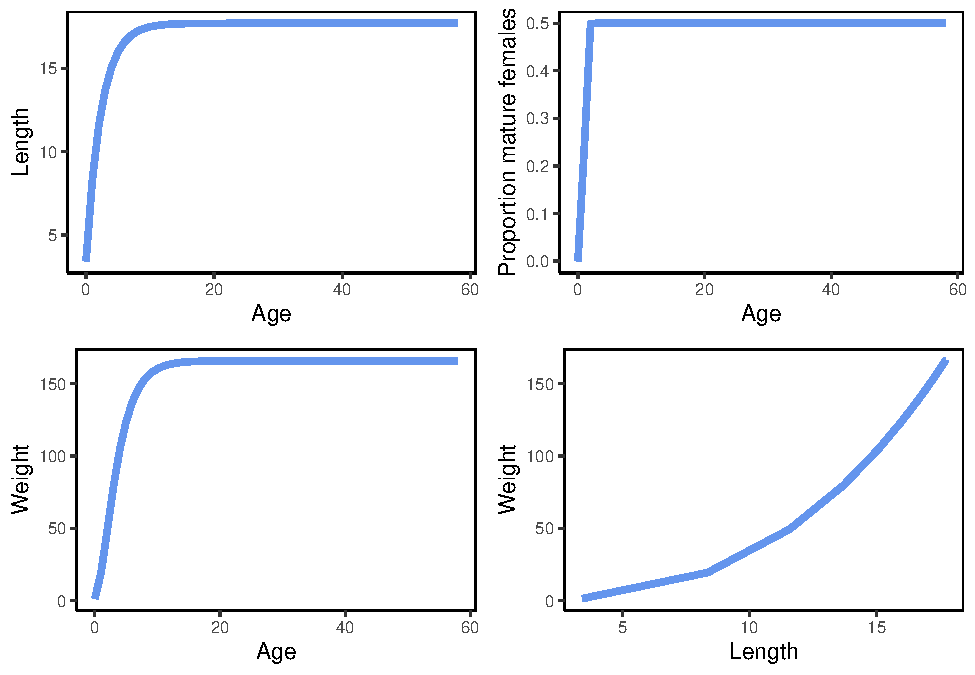
\includegraphics{_main_files/figure-latex/lifehist-1.pdf}
\caption{\label{fig:lifehist}Life history schedules.}
\end{figure}

The upper panels represent the von Bertalanffy growth curve (left) and the maturity ogive (right). The bottom panels represent the weight-at-age relationship and the allometric length-weight relationship.

\texttt{lhOut} returns all the details of the life history.

\begin{Shaded}
\begin{Highlighting}[]
\CommentTok{\#To return life history details}
\NormalTok{lhOut}
\end{Highlighting}
\end{Shaded}

\begin{itemize}
\tightlist
\item
  Vulnerability, retention, keep, dead discards, and removals at length can be plotted using the \texttt{selWrapper()} function.
\end{itemize}

\begin{Shaded}
\begin{Highlighting}[]
\NormalTok{selOut}\OtherTok{\textless{}{-}}\FunctionTok{selWrapper}\NormalTok{(}\AttributeTok{lh =}\NormalTok{ lhOut, TimeAreaObj, }\AttributeTok{FisheryObj =}\NormalTok{ HistFisheryObj, }\AttributeTok{doPlot =} \ConstantTok{TRUE}\NormalTok{)}
\end{Highlighting}
\end{Shaded}

\begin{figure}
\centering
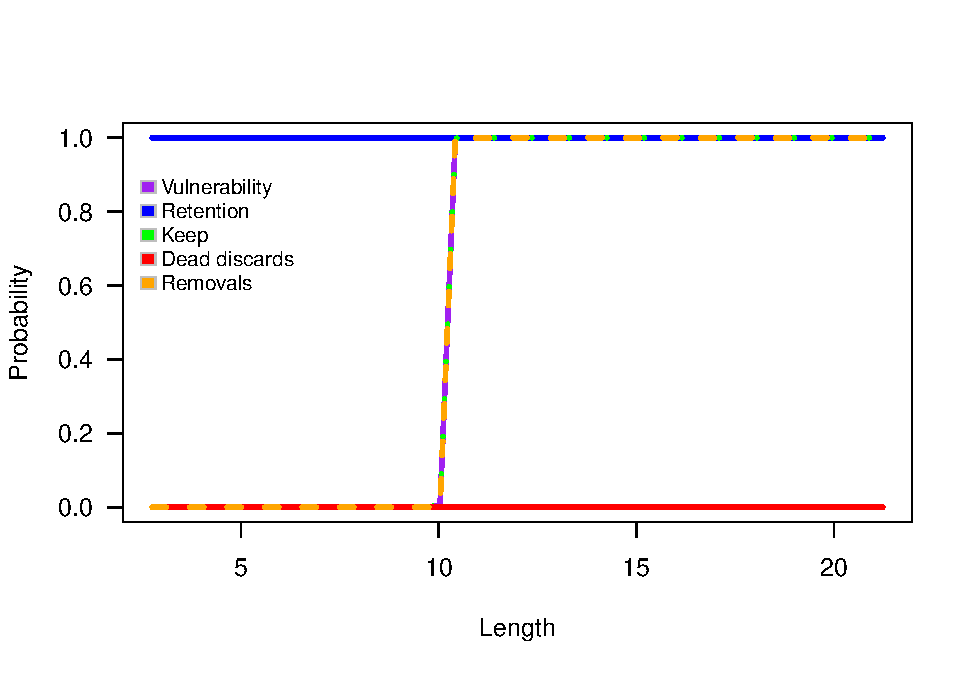
\includegraphics{_main_files/figure-latex/sel-1.pdf}
\caption{\label{fig:sel}Logistic selectivity function.}
\end{figure}

\texttt{selOut} returns all the details of the fishery selectivity.

\begin{Shaded}
\begin{Highlighting}[]
\CommentTok{\#To return sel details}
\NormalTok{selOut}
\end{Highlighting}
\end{Shaded}

If the user modifies the vulnerability, retention, and discard parameters in the \texttt{HistFisheryObj}, other selectivity/vulnerability and retention shapes can be explored. For example:

-- Assuming a vulnerability type \texttt{vulType} of ``explog'', with parameters p1, peak, and p3.

\begin{Shaded}
\begin{Highlighting}[]
\NormalTok{HistFisheryObj}\SpecialCharTok{@}\NormalTok{vulType}\OtherTok{\textless{}{-}}\StringTok{"explog"}
\NormalTok{HistFisheryObj}\SpecialCharTok{@}\NormalTok{vulParams}\OtherTok{\textless{}{-}}\FunctionTok{c}\NormalTok{(}\FloatTok{0.9}\NormalTok{,}\DecValTok{10}\NormalTok{,}\FloatTok{0.15}\NormalTok{) }\CommentTok{\#dome{-}shaped}
\NormalTok{HistFisheryObj}\SpecialCharTok{@}\NormalTok{retType}\OtherTok{\textless{}{-}}\StringTok{"full"}
\NormalTok{HistFisheryObj}\SpecialCharTok{@}\NormalTok{retMax }\OtherTok{\textless{}{-}} \DecValTok{1}
\NormalTok{HistFisheryObj}\SpecialCharTok{@}\NormalTok{Dmort }\OtherTok{\textless{}{-}} \DecValTok{0}
\NormalTok{selOut}\OtherTok{\textless{}{-}}\FunctionTok{selWrapper}\NormalTok{(}\AttributeTok{lh =}\NormalTok{ lhOut, TimeAreaObj, }\AttributeTok{FisheryObj =}\NormalTok{ HistFisheryObj, }\AttributeTok{doPlot =} \ConstantTok{TRUE}\NormalTok{)}
\end{Highlighting}
\end{Shaded}

\begin{figure}
\centering
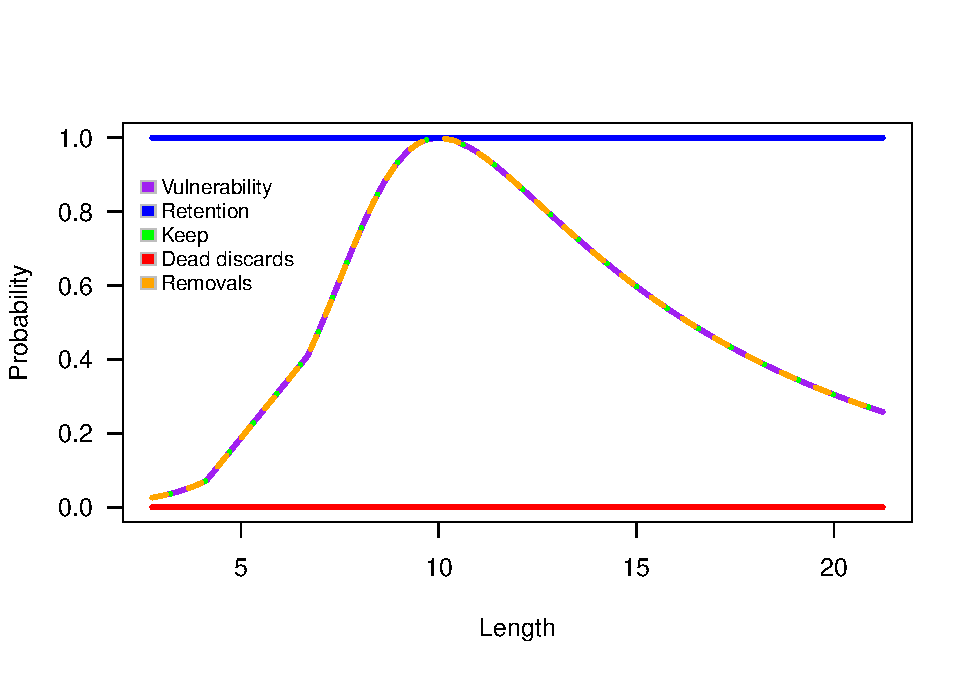
\includegraphics{_main_files/figure-latex/sel2-1.pdf}
\caption{\label{fig:sel2}Exponential logistic selectivity (dome-shaped).}
\end{figure}

-- Assuming a vulnerability type \texttt{vulType} of ``logistic'', with changes in the retention type (\texttt{retType}) and retention parameters (\texttt{retParams}).

\begin{Shaded}
\begin{Highlighting}[]
\NormalTok{HistFisheryObj}\SpecialCharTok{@}\NormalTok{vulType}\OtherTok{\textless{}{-}}\StringTok{"logistic"}
\NormalTok{HistFisheryObj}\SpecialCharTok{@}\NormalTok{vulParams}\OtherTok{\textless{}{-}}\FunctionTok{c}\NormalTok{(}\FloatTok{10.2}\NormalTok{,}\FloatTok{0.1}\NormalTok{) }\CommentTok{\#Approx. knife edge}
\NormalTok{HistFisheryObj}\SpecialCharTok{@}\NormalTok{retType}\OtherTok{\textless{}{-}}\StringTok{"logistic"}
\NormalTok{HistFisheryObj}\SpecialCharTok{@}\NormalTok{retParams}\OtherTok{\textless{}{-}}\FunctionTok{c}\NormalTok{(}\DecValTok{11}\NormalTok{,}\FloatTok{0.8}\NormalTok{)}
\NormalTok{HistFisheryObj}\SpecialCharTok{@}\NormalTok{retMax }\OtherTok{\textless{}{-}} \DecValTok{1}
\NormalTok{HistFisheryObj}\SpecialCharTok{@}\NormalTok{Dmort }\OtherTok{\textless{}{-}} \DecValTok{0}
\NormalTok{selOut}\OtherTok{\textless{}{-}}\FunctionTok{selWrapper}\NormalTok{(}\AttributeTok{lh =}\NormalTok{ lhOut, TimeAreaObj, }\AttributeTok{FisheryObj =}\NormalTok{ HistFisheryObj, }\AttributeTok{doPlot =} \ConstantTok{TRUE}\NormalTok{)}
\end{Highlighting}
\end{Shaded}

\begin{figure}
\centering
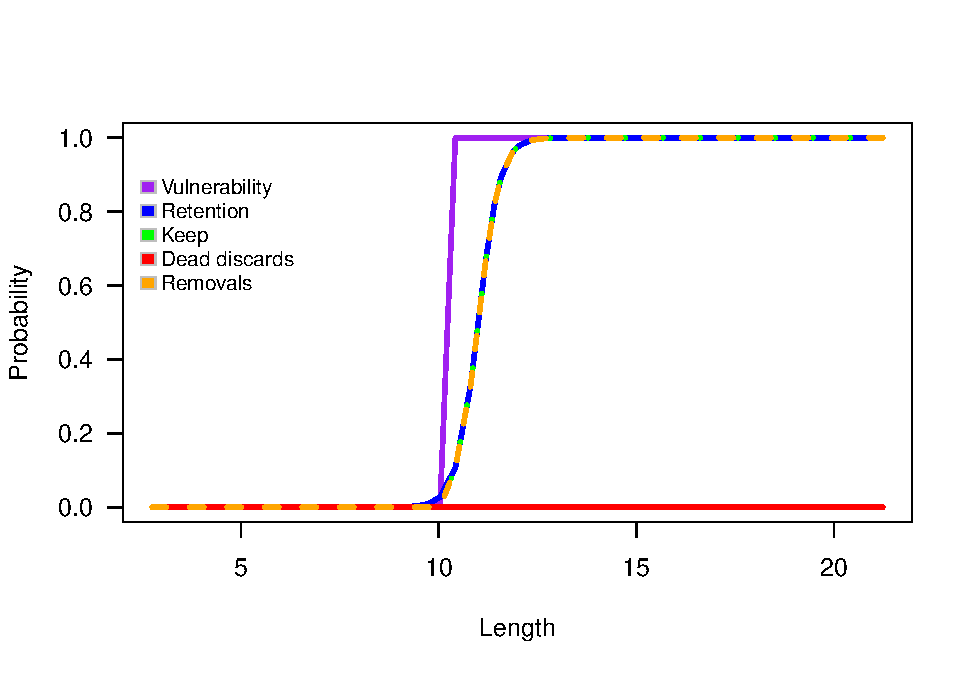
\includegraphics{_main_files/figure-latex/sel3-1.pdf}
\caption{\label{fig:sel3}Logistic selectivity function with different retention parameters.}
\end{figure}

-- Assuming a vulnerability type \texttt{vulType} of ``gillnetMasterNormal'' with parameters (\texttt{vulParams}), represented as \texttt{c(p1,\ p2,\ and\ p3)} and changes in the retention type (\texttt{retType}) and retention parameters (\texttt{retParams}).

\begin{Shaded}
\begin{Highlighting}[]
\NormalTok{HistFisheryObj}\SpecialCharTok{@}\NormalTok{vulType}\OtherTok{\textless{}{-}}\StringTok{"gillnetMasterNormal"}
\NormalTok{HistFisheryObj}\SpecialCharTok{@}\NormalTok{vulParams}\OtherTok{\textless{}{-}}\FunctionTok{c}\NormalTok{(}\FloatTok{2.5}\NormalTok{,}\FloatTok{0.1}\NormalTok{,}\DecValTok{4}\NormalTok{)}
\NormalTok{HistFisheryObj}\SpecialCharTok{@}\NormalTok{retType}\OtherTok{\textless{}{-}}\StringTok{"logistic"}
\NormalTok{HistFisheryObj}\SpecialCharTok{@}\NormalTok{retParams}\OtherTok{\textless{}{-}}\FunctionTok{c}\NormalTok{(}\DecValTok{9}\NormalTok{,}\FloatTok{0.5}\NormalTok{)}
\NormalTok{HistFisheryObj}\SpecialCharTok{@}\NormalTok{retMax }\OtherTok{\textless{}{-}} \DecValTok{1}
\NormalTok{HistFisheryObj}\SpecialCharTok{@}\NormalTok{Dmort }\OtherTok{\textless{}{-}} \DecValTok{0}
\NormalTok{selOut}\OtherTok{\textless{}{-}}\FunctionTok{selWrapper}\NormalTok{(}\AttributeTok{lh =}\NormalTok{ lhOut, TimeAreaObj, }\AttributeTok{FisheryObj =}\NormalTok{ HistFisheryObj, }\AttributeTok{doPlot =} \ConstantTok{TRUE}\NormalTok{)}
\end{Highlighting}
\end{Shaded}

\begin{figure}
\centering
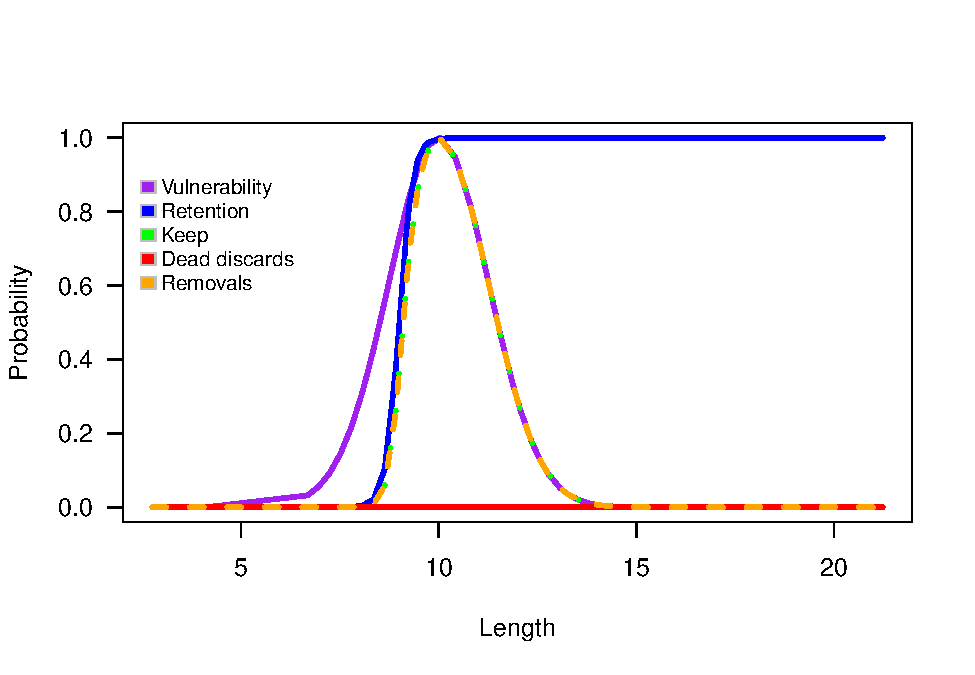
\includegraphics{_main_files/figure-latex/sel4-1.pdf}
\caption{\label{fig:sel4}Gillnet master normal selectivity function with different retention parameters.}
\end{figure}

-- Assuming a vulnerability type \texttt{vulType} of ``gillnetMasterLognormal'' with parameters (\texttt{vulParams}), represented as \texttt{c(p1,\ p2,\ and\ p3)} and changes in the retention type (\texttt{retType}) and retention parameters (\texttt{retParams}).

\begin{Shaded}
\begin{Highlighting}[]
\NormalTok{HistFisheryObj}\SpecialCharTok{@}\NormalTok{vulType}\OtherTok{\textless{}{-}}\StringTok{"gillnetMasterLognormal"}
\NormalTok{HistFisheryObj}\SpecialCharTok{@}\NormalTok{vulParams}\OtherTok{\textless{}{-}}\FunctionTok{c}\NormalTok{(}\FloatTok{2.5}\NormalTok{,}\FloatTok{0.1}\NormalTok{,}\DecValTok{4}\NormalTok{)}
\NormalTok{HistFisheryObj}\SpecialCharTok{@}\NormalTok{retType}\OtherTok{\textless{}{-}}\StringTok{"logistic"}
\NormalTok{HistFisheryObj}\SpecialCharTok{@}\NormalTok{retParams}\OtherTok{\textless{}{-}}\FunctionTok{c}\NormalTok{(}\DecValTok{9}\NormalTok{,}\FloatTok{0.5}\NormalTok{)}
\NormalTok{HistFisheryObj}\SpecialCharTok{@}\NormalTok{retMax }\OtherTok{\textless{}{-}} \DecValTok{1}
\NormalTok{HistFisheryObj}\SpecialCharTok{@}\NormalTok{Dmort }\OtherTok{\textless{}{-}} \DecValTok{0}
\NormalTok{selOut}\OtherTok{\textless{}{-}}\FunctionTok{selWrapper}\NormalTok{(}\AttributeTok{lh =}\NormalTok{ lhOut, TimeAreaObj, }\AttributeTok{FisheryObj =}\NormalTok{ HistFisheryObj, }\AttributeTok{doPlot =} \ConstantTok{TRUE}\NormalTok{)}
\end{Highlighting}
\end{Shaded}

\begin{figure}
\centering
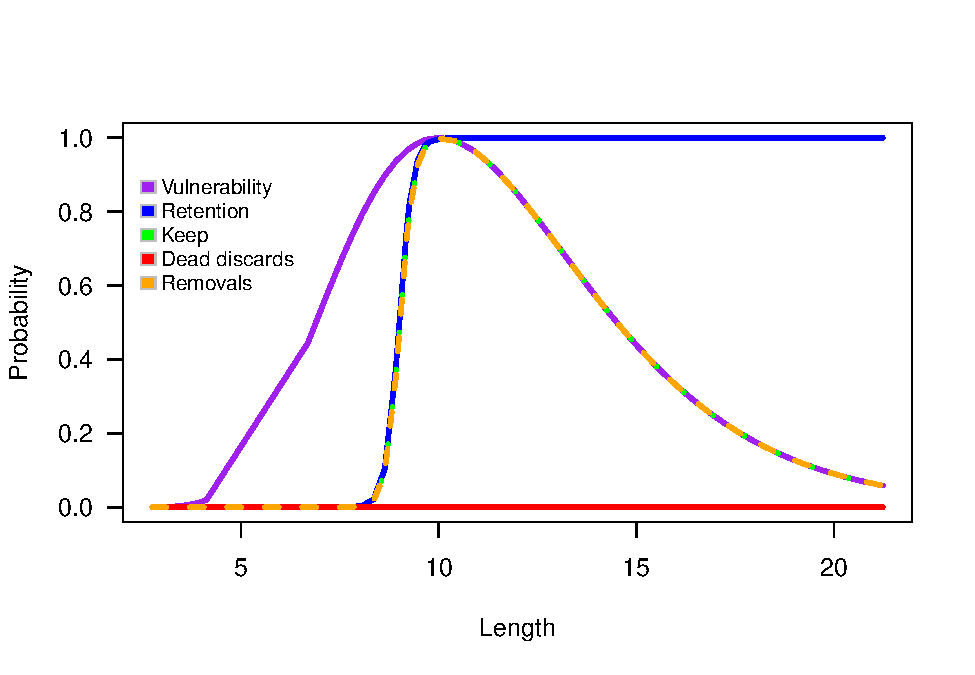
\includegraphics{_main_files/figure-latex/sel5-1.pdf}
\caption{\label{fig:sel5}Gillnet master log normal selectivity function with different retention parameters.}
\end{figure}

\section{Stochastic object}\label{stochastic-object}

The \texttt{StochasticObj} holds the parameters for stochastic components of the population and fishery dynamics.
To create a new object of class \texttt{Stochastic}, use the \texttt{new()} function.

\begin{Shaded}
\begin{Highlighting}[]
\NormalTok{StochasticObj}\OtherTok{\textless{}{-}}\FunctionTok{new}\NormalTok{(}\StringTok{"Stochastic"}\NormalTok{)}
\end{Highlighting}
\end{Shaded}

Similar to other S4 objects, the slot names of \texttt{StochasticObj} can be viewed using the \texttt{slotNames()} function, and the help file can be accessed using the \texttt{?} symbol.

\begin{Shaded}
\begin{Highlighting}[]
\FunctionTok{slotNames}\NormalTok{(StochasticObj)}
\end{Highlighting}
\end{Shaded}

\begin{verbatim}
##  [1] "title"                "historicalBio"        "Linf"                
##  [4] "K"                    "L50"                  "L95delta"            
##  [7] "M"                    "Steep"                "recSD"               
## [10] "recRho"               "H50"                  "H95delta"            
## [13] "histFisheryVul"       "proFisheryVul_list"   "sameFisheryVul"      
## [16] "histFisheryRet"       "proFisheryRet_list"   "sameFisheryRet"      
## [19] "histFisheryDmort"     "proFisheryDmort_list" "sameFisheryDmort"
\end{verbatim}

\begin{Shaded}
\begin{Highlighting}[]
\CommentTok{\#getting help}
\NormalTok{?}\StringTok{\textasciigrave{}}\AttributeTok{Stochastic{-}class}\StringTok{\textasciigrave{}}  
\end{Highlighting}
\end{Shaded}

To populate the slots of \texttt{StochasticObj}, the user should begin by defining a meaningful title (\texttt{title}) and specifying the parameters in which they want to include stochasticity.

The slots defined in the \texttt{StochasticObj} object create additional inputs and override parameters specified elsewhere (e.g., \texttt{LifeHistoryObj}, \texttt{HistFisheryObj}, or \texttt{TimeAreaObj}), allowing the corresponding model components to become stochastic. The exception is recruitment variation (\texttt{recSD}), which is entered in the \texttt{LifeHistoryObj} object.

In the following example, we add uncertainty to \texttt{historicalBio} by replacing the parameter defined in the \texttt{TimeAreaObj} object (\texttt{TimeArea@historicalBio}) with a vector of length 2 that contains the lower and upper bounds of a uniform distribution for the historical equilibrium biomass \texttt{historicalBio}. During each iteration, one value is drawn from the uniform distribution.

\begin{Shaded}
\begin{Highlighting}[]
\NormalTok{StochasticObj}\SpecialCharTok{@}\NormalTok{title}\OtherTok{\textless{}{-}}\StringTok{"adding unceratinty"}
\NormalTok{StochasticObj}\SpecialCharTok{@}\NormalTok{historicalBio }\OtherTok{=} \FunctionTok{c}\NormalTok{(}\FloatTok{0.3}\NormalTok{, }\FloatTok{0.6}\NormalTok{)}
\end{Highlighting}
\end{Shaded}

\subsection{\texorpdfstring{Adding stochasticity to the \texttt{LifeHistoryObj} object}{Adding stochasticity to the LifeHistoryObj object}}\label{adding-stochasticity-to-the-lifehistoryobj-object}

All scalar parameters in the \texttt{LifeHistoryObj} object that hold a single value, such as \texttt{Linf}, \texttt{K}, \texttt{L50}, \texttt{L95delta}, \texttt{M}, \texttt{Steep}, \texttt{recSD}, \texttt{recRho}, \texttt{H50}, and \texttt{H95delta}, can be redefined in the \texttt{StochasticObj} object. When redefined, they are replaced by a vector of length 2 containing the minimum and maximum values. If provided, these values override those in the \texttt{LifeHistoryObj}, and a unique value for each iteration is generated by sampling from the uniform distribution.

\begin{Shaded}
\begin{Highlighting}[]
\NormalTok{StochasticObj}\SpecialCharTok{@}\NormalTok{Steep }\OtherTok{=} \FunctionTok{c}\NormalTok{(}\FloatTok{0.5}\NormalTok{, }\FloatTok{0.6}\NormalTok{) }\CommentTok{\#e.g., adding stochasticity to Steepness}
\end{Highlighting}
\end{Shaded}

\subsection{\texorpdfstring{Adding stochasticity to the \texttt{HistFisheryObj} object}{Adding stochasticity to the HistFisheryObj object}}\label{adding-stochasticity-to-the-histfisheryobj-object}

A matrix with \(n\) columns and 2 rows is used to define the range of uncertainty for the vulnerability (\texttt{vulParams}) and retention (\texttt{retParams}) parameters from the \texttt{HistFisheryObj} in the \texttt{StochasticObj} object. Row 1 contains the minimum values, and row 2 contains the maximum values for each parameter, corresponding to the respective column \(n\).

When this matrix is provided in the \texttt{StochasticObj} object, it replaces the \texttt{vulParams} and \texttt{retParams} slots previously defined in the \texttt{HistFisheryObj}. This ensures that the columns of the matrix align with the required inputs for \texttt{vulType} and \texttt{retType} in the \texttt{HistFisheryObj} object.

The same logic applies to redefining the \texttt{Dmort} parameter, but in this case, the matrix contains only 1 column and 2 rows (min and max), as the \texttt{Dmort} parameter is a scalar. When this matrix is provided, it replaces the \texttt{Dmort} slot in the \texttt{HistFisheryObj}.

\begin{Shaded}
\begin{Highlighting}[]
\NormalTok{StochasticObj}\SpecialCharTok{@}\NormalTok{histFisheryVul}\OtherTok{=}\FunctionTok{matrix}\NormalTok{(}\FunctionTok{c}\NormalTok{(}\DecValTok{9}\NormalTok{,}\DecValTok{11}\NormalTok{,}\FloatTok{0.07}\NormalTok{,}\FloatTok{0.13}\NormalTok{), }\AttributeTok{nrow=}\DecValTok{2}\NormalTok{, }\AttributeTok{ncol=}\DecValTok{2}\NormalTok{,}\AttributeTok{byrow=}\ConstantTok{FALSE}\NormalTok{)  }\CommentTok{\#e.g., adding stochasticity to histFisheryVul}
\end{Highlighting}
\end{Shaded}

There are additional slots in the \texttt{StochasticObj} object that modify fishery projections (\texttt{ProFisheryObj}), which will be described in detail in a separate section.

\section{Fishery projections}\label{fishery-projections}

The user has the option to modify the \texttt{HistFisheryObj} object when performing fishery projections. These modifications are stored in \texttt{ProFisheryObj}. The slots of \texttt{ProFisheryObj} can either be set to the same values as those in \texttt{HistFisheryObj} or adjusted to modify vulnerability, retention, and discard scenarios during the projection phase.

\texttt{ProFisheryObj} can be populated as follows:

\begin{Shaded}
\begin{Highlighting}[]
\NormalTok{ProFisheryObj}\OtherTok{\textless{}{-}}\FunctionTok{new}\NormalTok{(}\StringTok{"Fishery"}\NormalTok{)}
\NormalTok{ProFisheryObj}\SpecialCharTok{@}\NormalTok{title}\OtherTok{\textless{}{-}}\StringTok{"Test"}
\NormalTok{ProFisheryObj}\SpecialCharTok{@}\NormalTok{vulType}\OtherTok{\textless{}{-}}\StringTok{"logistic"}
\NormalTok{ProFisheryObj}\SpecialCharTok{@}\NormalTok{vulParams}\OtherTok{\textless{}{-}}\FunctionTok{c}\NormalTok{(}\FloatTok{10.2}\NormalTok{,}\FloatTok{0.1}\NormalTok{)}
\NormalTok{ProFisheryObj}\SpecialCharTok{@}\NormalTok{retType}\OtherTok{\textless{}{-}}\StringTok{"logistic"}
\NormalTok{ProFisheryObj}\SpecialCharTok{@}\NormalTok{retParams }\OtherTok{\textless{}{-}} \FunctionTok{c}\NormalTok{(}\FloatTok{10.2}\NormalTok{, }\FloatTok{0.1}\NormalTok{)}
\NormalTok{ProFisheryObj}\SpecialCharTok{@}\NormalTok{retMax }\OtherTok{\textless{}{-}} \DecValTok{1}
\NormalTok{ProFisheryObj}\SpecialCharTok{@}\NormalTok{Dmort }\OtherTok{\textless{}{-}} \DecValTok{0}
\end{Highlighting}
\end{Shaded}

In this example, during the projections, we maintain the same vulnerability type and parameters as in the \texttt{HistFisheryObj} object but modify retention to follow a logistic function, using the same parameters as vulnerability.

\subsection{Adding stochasticity to the fishery projections}\label{adding-stochasticity-to-the-fishery-projections}

Additional slots in the \texttt{StochasticObj} object allow for modifications to the fishery projections (\texttt{ProFisheryObj}). These additional slots, \texttt{proFisheryVul\_list}, \texttt{proFisheryRet\_list}, and \texttt{proFisheryDmort\_list}, are lists where the number of objects corresponds to the number of areas (\texttt{TimeAreaObj@areas}) defined in the model. Each object in the list is a matrix with \(n\) columns and 2 rows, where the rows represent the minimum and maximum values for the parameters associated with each column \(n\).

When provided, these lists replace the \texttt{vulParams}, \texttt{retParams}, and \texttt{Dmort} slots in the fishery projections (\texttt{ProFisheryObj}). For \texttt{proFisheryVul\_list} and \texttt{proFisheryRet\_list}, the columns of the matrix align with the required inputs for \texttt{ProFisheryObj@vulType} and \texttt{ProFisheryObj@retType}.

During each iteration, the model samples values from a uniform distribution within the specified range (i.e., between the min and max values in each row), allowing for stochastic variation in the parameters across different areas.

The final slots in the \texttt{StochasticObj} object are \texttt{sameFisheryVul}, \texttt{sameFisheryRet}, and \texttt{sameFisheryDmort}. These slots determine whether the historical and projection parameter values for vulnerability, retention, and discards remain identical. Each slot contains a logical variable (``TRUE'' or ``FALSE'') that specifies whether the values defined in the \texttt{HistFisheryObj} for \texttt{vulParams}, \texttt{retParams}, and \texttt{Dmort} should also be applied to the fishery projections (\texttt{ProFisheryObj}) for \texttt{vulType}, \texttt{retType}, and \texttt{Dmort}. If set to \texttt{TRUE}, this will override any input provided in \texttt{ProFisheryObj} for these slots.

\section{The management strategy}\label{the-management-strategy}

The management strategy (\texttt{StrategyObj}) holds descriptions of projections to be made, including a harvest strategy. One of the most distinctive features of \textbf{FishSimGTG} is that it allows the user to customize the desired management procedures.

To create a new object of class \texttt{StrategyObj}, use the \texttt{new()} function.

\begin{Shaded}
\begin{Highlighting}[]
\NormalTok{StrategyObj}\OtherTok{\textless{}{-}}\FunctionTok{new}\NormalTok{(}\StringTok{"Strategy"}\NormalTok{)}
\end{Highlighting}
\end{Shaded}

To populate the \texttt{StrategyObj}, the user should start by specifying the number of forward projection years to simulate (\texttt{projectionYears}), the \texttt{projectionName}, which defines the name of the strategy, and \texttt{projectionParams}, a list structure that follows the specifications of the projection function defined in \texttt{projectionName}.

In this example, \texttt{projectionParams} is a list with four items. The first item is a vector of length \texttt{areas} containing bag limits (\texttt{bag}). To indicate no bag limit, use \texttt{-99}. The bag limit should be considered as the take per unit time (e.g., per day) and basically acts like a CPUE threshold.

The second item is a matrix with \texttt{nrows\ =\ projectionYears} and \texttt{ncols\ =\ areas} that contains value multipliers of the initial equilibrium fishing effort (\texttt{effort}). This allows for the projection of effort reductions and the establishment of marine reserves by setting effort to \texttt{0}.

The two final items are a vector of length \texttt{areas} containing CPUE (\texttt{CPUE}), along with a \texttt{CPUEtype}, which is defined as a character string (e.g., \texttt{retN} for retention in numbers).

\begin{Shaded}
\begin{Highlighting}[]
\NormalTok{StrategyObj}\SpecialCharTok{@}\NormalTok{projectionYears }\OtherTok{\textless{}{-}} \DecValTok{50}
\NormalTok{StrategyObj}\SpecialCharTok{@}\NormalTok{projectionName}\OtherTok{\textless{}{-}}\StringTok{"projectionStrategy"}
\NormalTok{StrategyObj}\SpecialCharTok{@}\NormalTok{projectionParams}\OtherTok{\textless{}{-}}\FunctionTok{list}\NormalTok{(}\AttributeTok{bag =} \FunctionTok{c}\NormalTok{(}\DecValTok{5}\NormalTok{, }\DecValTok{5}\NormalTok{), }\AttributeTok{effort =} \FunctionTok{matrix}\NormalTok{(}\DecValTok{1}\SpecialCharTok{:}\DecValTok{1}\NormalTok{, }\AttributeTok{nrow=}\DecValTok{50}\NormalTok{, }\AttributeTok{ncol=}\DecValTok{2}\NormalTok{, }\AttributeTok{byrow =} \ConstantTok{FALSE}\NormalTok{), }\AttributeTok{CPUE =} \FunctionTok{c}\NormalTok{(}\DecValTok{7}\NormalTok{,}\DecValTok{11}\NormalTok{), }\AttributeTok{CPUEtype =} \StringTok{\textquotesingle{}retN\textquotesingle{}}\NormalTok{)}
\end{Highlighting}
\end{Shaded}

\section{Running the projection and management strategy simulation}\label{running-the-projection-and-management-strategy-simulation}

This section provides an example for the user on how to run projections using three management strategies that combine minimum size and bag limits.

\begin{Shaded}
\begin{Highlighting}[]
\CommentTok{\#Batch processing {-} 3 management strategies}
\NormalTok{stateLmin}\OtherTok{\textless{}{-}}\FunctionTok{c}\NormalTok{(}\FloatTok{10.2}\NormalTok{, }\FloatTok{12.7}\NormalTok{,  }\FloatTok{12.7}\NormalTok{)}
\NormalTok{stateBag}\OtherTok{\textless{}{-}}\FunctionTok{c}\NormalTok{(}\DecValTok{20}\NormalTok{, }\SpecialCharTok{{-}}\DecValTok{99}\NormalTok{, }\DecValTok{20}\NormalTok{)}
\NormalTok{fileLabel}\OtherTok{\textless{}{-}}\FunctionTok{c}\NormalTok{(}\StringTok{"Higher\_option1"}\NormalTok{, }\StringTok{"Higher\_option2"}\NormalTok{, }\StringTok{"Higher\_option3"}\NormalTok{)}
\NormalTok{projectionLabel}\OtherTok{\textless{}{-}}\FunctionTok{c}\NormalTok{(}\StringTok{"Bag 20"}\NormalTok{, }\StringTok{"Min size 5 inch"}\NormalTok{, }\StringTok{"Bag 20 \& min size 5 inch"}\NormalTok{)}
\end{Highlighting}
\end{Shaded}

In this example, \texttt{stateLmin} is a vector containing three minimum sizes, and \texttt{stateBag} is a vector that contains three bag limits. To indicate no bag limit, use \texttt{-99}. \texttt{fileLabel} is a label for the file name, and \texttt{projectionLabel} defines the name for the strategy that will be evaluated.

To run the projection under the three different management strategies (i.e., ``Bag 20'', ``Min size 5 inch'', and ``Bag 20 \& Min size 5 inch''), we will use the \texttt{runProjection()}.

In this example, we modify the retention parameters of the logistic function previously defined in \texttt{ProFisheryObj@retParams}. These parameters are now redefined as \texttt{ProFisheryObj@retParams\ \textless{}-\ c(stateLmin{[}sc{]},\ 0.1)}, using the pre-specified size limits (\texttt{stateLmin}).

Additionally, in the list structure of the \texttt{StrategyObj@projectionParams}, the elements of the \texttt{bag} vector are replaced by the specified bag limits (\texttt{stateBag}).

\begin{Shaded}
\begin{Highlighting}[]
\ControlFlowTok{for}\NormalTok{(sc }\ControlFlowTok{in} \DecValTok{1}\SpecialCharTok{:}\FunctionTok{NROW}\NormalTok{(stateLmin))\{}

  \CommentTok{\#Size limit {-} changes retention, not selectivity}
\NormalTok{  ProFisheryObj}\SpecialCharTok{@}\NormalTok{retParams}\OtherTok{\textless{}{-}}\FunctionTok{c}\NormalTok{(stateLmin[sc],}\FloatTok{0.1}\NormalTok{)}

  \CommentTok{\#Bag limit}
\NormalTok{StrategyObj}\SpecialCharTok{@}\NormalTok{projectionParams}\OtherTok{\textless{}{-}}\FunctionTok{list}\NormalTok{(}\AttributeTok{bag =} \FunctionTok{c}\NormalTok{(stateBag[sc], stateBag[sc]), }\AttributeTok{effort =} \FunctionTok{matrix}\NormalTok{(}\DecValTok{1}\SpecialCharTok{:}\DecValTok{1}\NormalTok{, }\AttributeTok{nrow=}\DecValTok{50}\NormalTok{, }\AttributeTok{ncol=}\DecValTok{2}\NormalTok{, }\AttributeTok{byrow =} \ConstantTok{FALSE}\NormalTok{), }\AttributeTok{CPUE =} \FunctionTok{c}\NormalTok{(}\DecValTok{7}\NormalTok{,}\DecValTok{11}\NormalTok{), }\AttributeTok{CPUEtype =} \StringTok{\textquotesingle{}retN\textquotesingle{}}\NormalTok{)}

  \FunctionTok{runProjection}\NormalTok{(}\AttributeTok{LifeHistoryObj =}\NormalTok{ LifeHistoryObj,}
                \AttributeTok{TimeAreaObj =}\NormalTok{ TimeAreaObj,}
                \AttributeTok{HistFisheryObj =}\NormalTok{ HistFisheryObj,}
                \AttributeTok{ProFisheryObj\_list =} \FunctionTok{list}\NormalTok{(ProFisheryObj, ProFisheryObj),}
                \AttributeTok{StrategyObj =}\NormalTok{ StrategyObj,}
                \AttributeTok{StochasticObj =}\NormalTok{ StochasticObj,}
                \AttributeTok{wd =} \FunctionTok{here}\NormalTok{(}\StringTok{"data{-}test"}\NormalTok{, }\StringTok{"Kole"}\NormalTok{),}
                \AttributeTok{fileName =}\NormalTok{ fileLabel[sc],}
                \AttributeTok{doPlot =} \ConstantTok{TRUE}\NormalTok{,}
                \AttributeTok{titleStrategy =}\NormalTok{ projectionLabel[sc]}
\NormalTok{  )}
\NormalTok{\}}
\end{Highlighting}
\end{Shaded}

The \texttt{runProjection()} function contains several arguments. The objects \texttt{LifeHistoryObj}, \texttt{TimeAreaObj}, \texttt{HistFisheryObj}, \texttt{ProFisheryObj\_list}, and \texttt{StrategyObj} were defined above. Among these, \texttt{LifeHistoryObj}, \texttt{TimeAreaObj}, and \texttt{HistFisheryObj} are required. The objects \texttt{StochasticObj}, \texttt{ProFisheryObj\_list}, and \texttt{StrategyObj} are optional; however, \texttt{ProFisheryObj\_list} should be used when \texttt{StrategyObj} is specified.

The function requires \texttt{ProFisheryObj} to be entered as a list, allowing the user to modify vulnerability, retention, and discard scenarios during the projection phase across different areas.

The \texttt{wd} argument is required and sets the working directory where the outputs of the projection will be saved. In this example, ``Kole'' is a subfolder of ``data-test,'' so all plots will be stored in ``Kole.''

The \texttt{fileName} argument specifies the output file name and can be set to the \texttt{fileLabel} defined above. This argument is always required.

The \texttt{doPlot} argument is a logical value indicating whether to produce diagnostic plots upon completing simulations. The default is \texttt{FALSE} (no plots).

The \texttt{titleStrategy} argument describes the title for the management strategy being evaluated and can be set to the \texttt{projectionLabel}.

To explore all the arguments of this function, the user can use \texttt{?ProFisheryObj}.

Next, we present some of the plots produced by \texttt{runProjection()}.

\begin{figure}
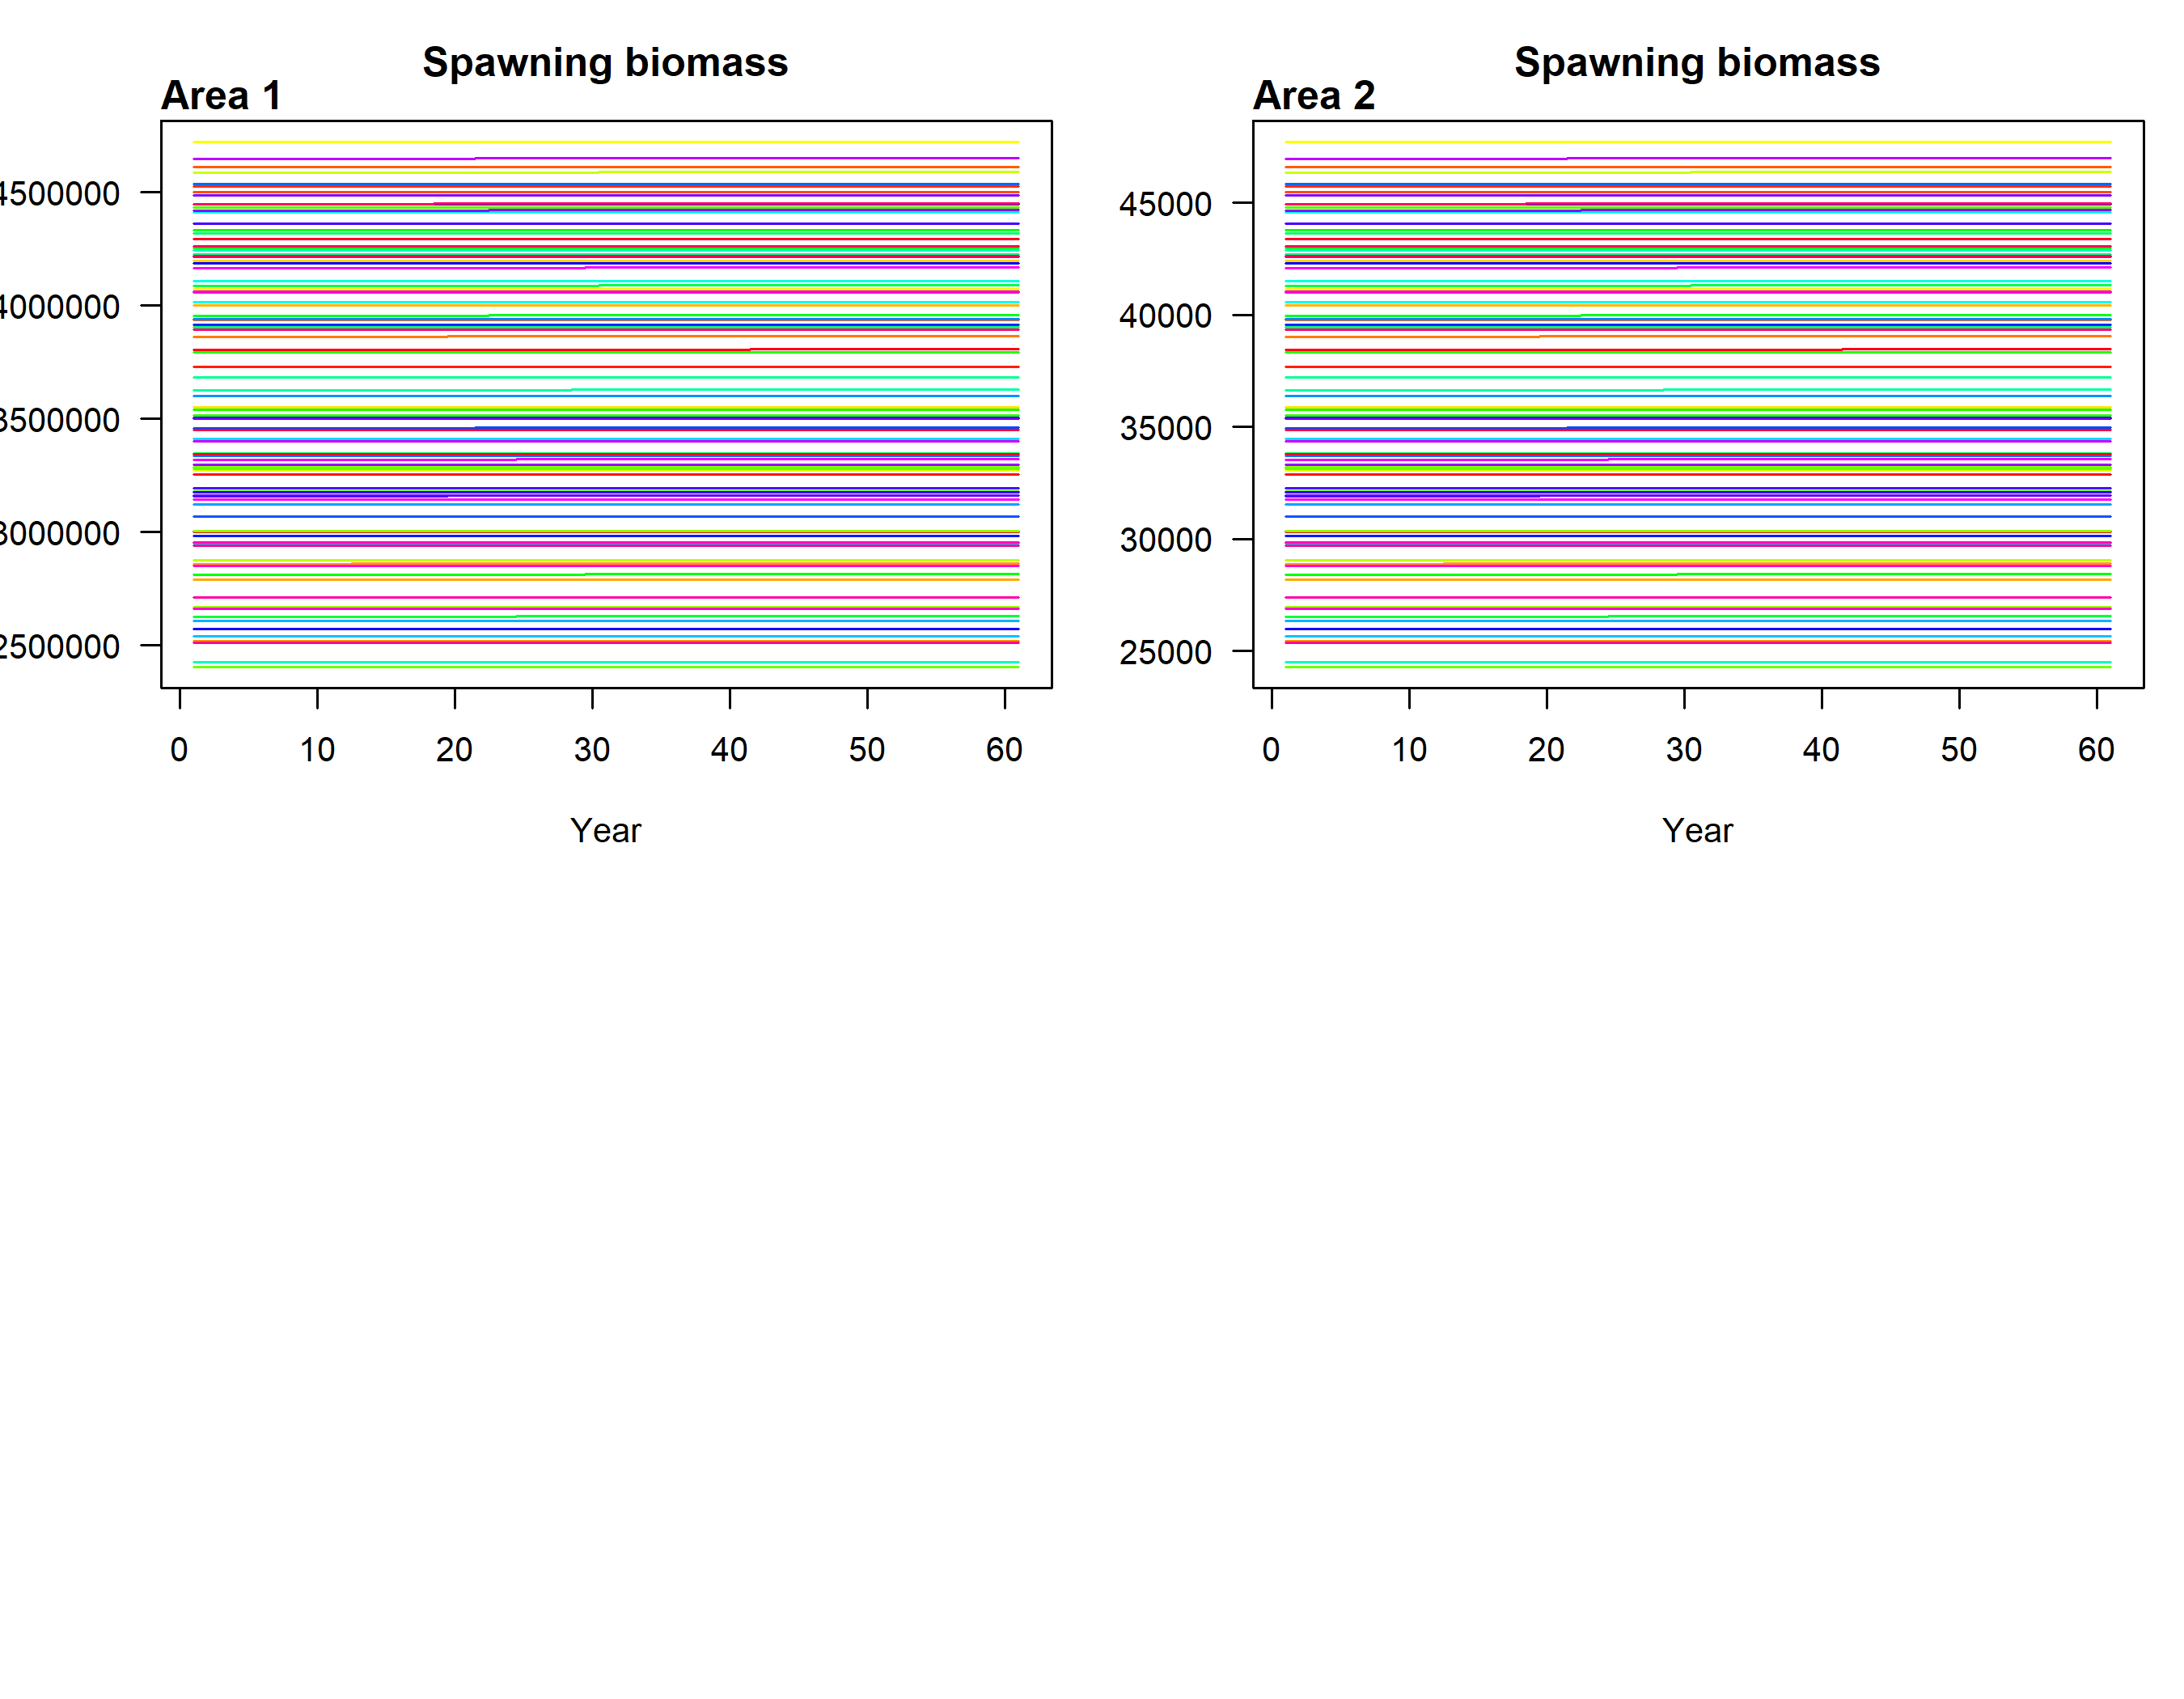
\includegraphics[width=1\linewidth]{data-test/Kole/Higher_option1_SB_Area} \caption{Spawning biomass by area- Higher_option1 }\label{fig:fig-SB-H-opt1}
\end{figure}

\begin{figure}
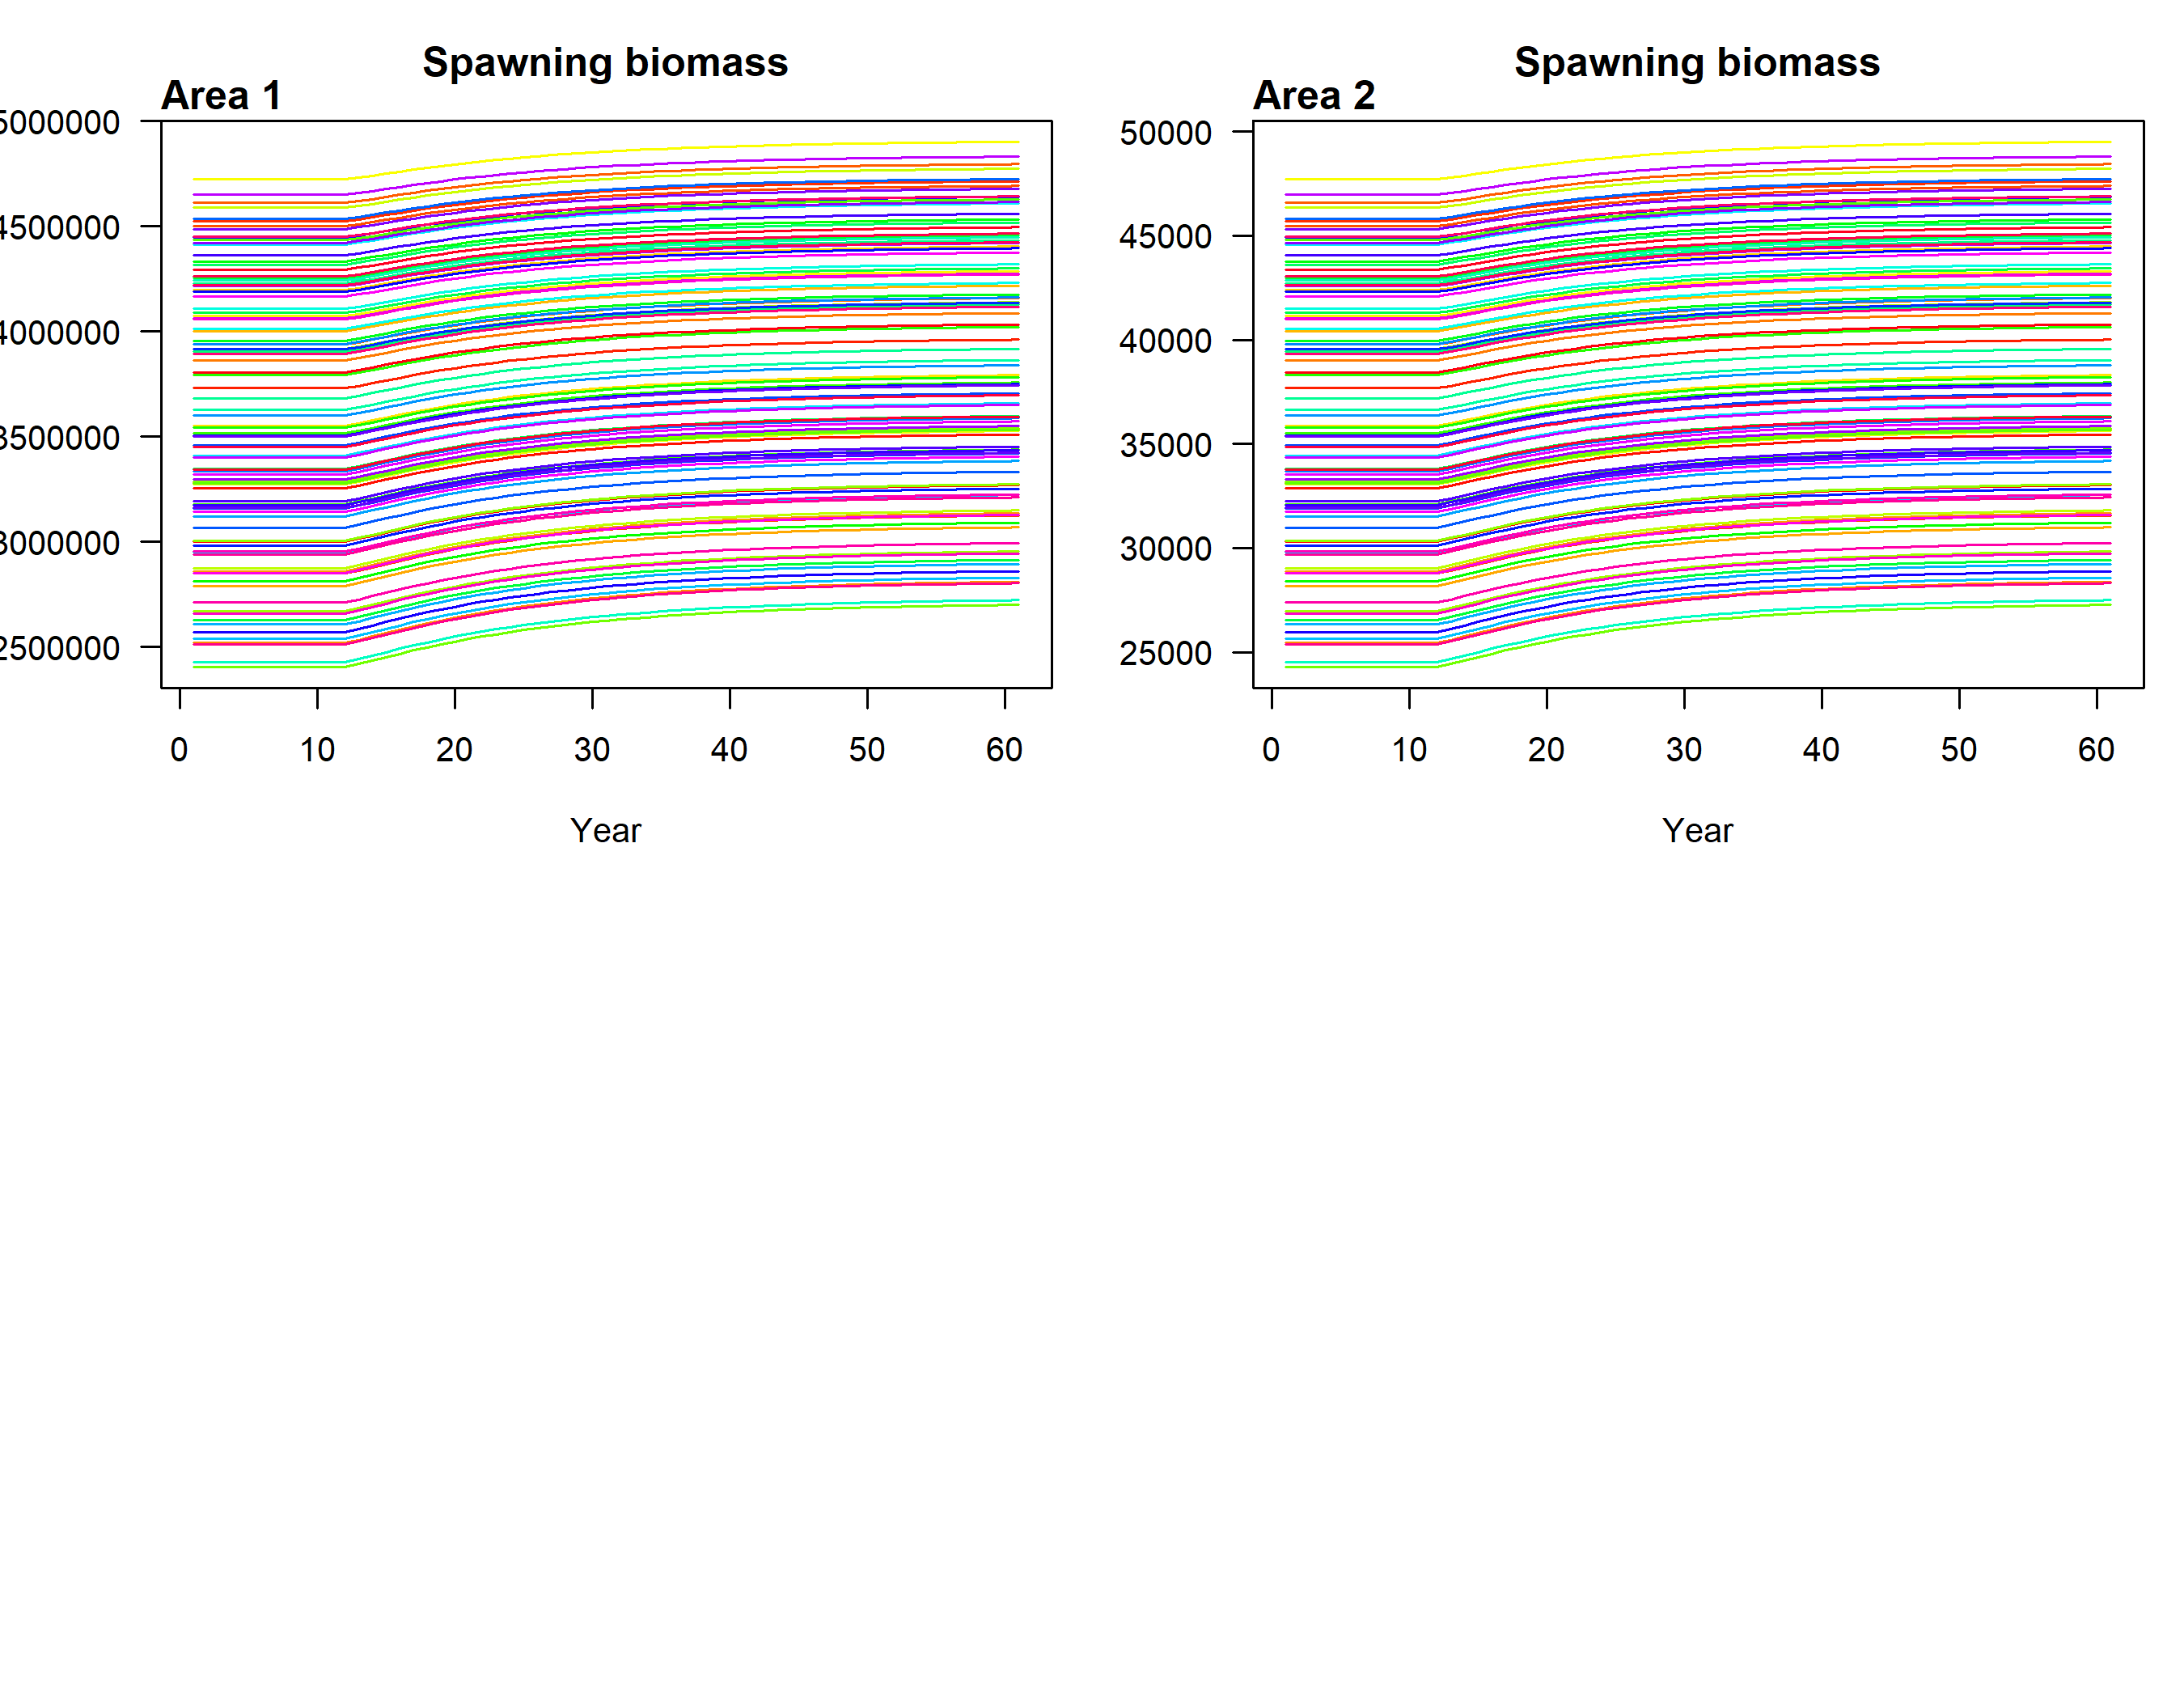
\includegraphics[width=1\linewidth]{data-test/Kole/Higher_option2_SB_Area} \caption{Spawning biomass by area- Higher_option2 }\label{fig:fig-SB-H-opt2}
\end{figure}

\begin{figure}
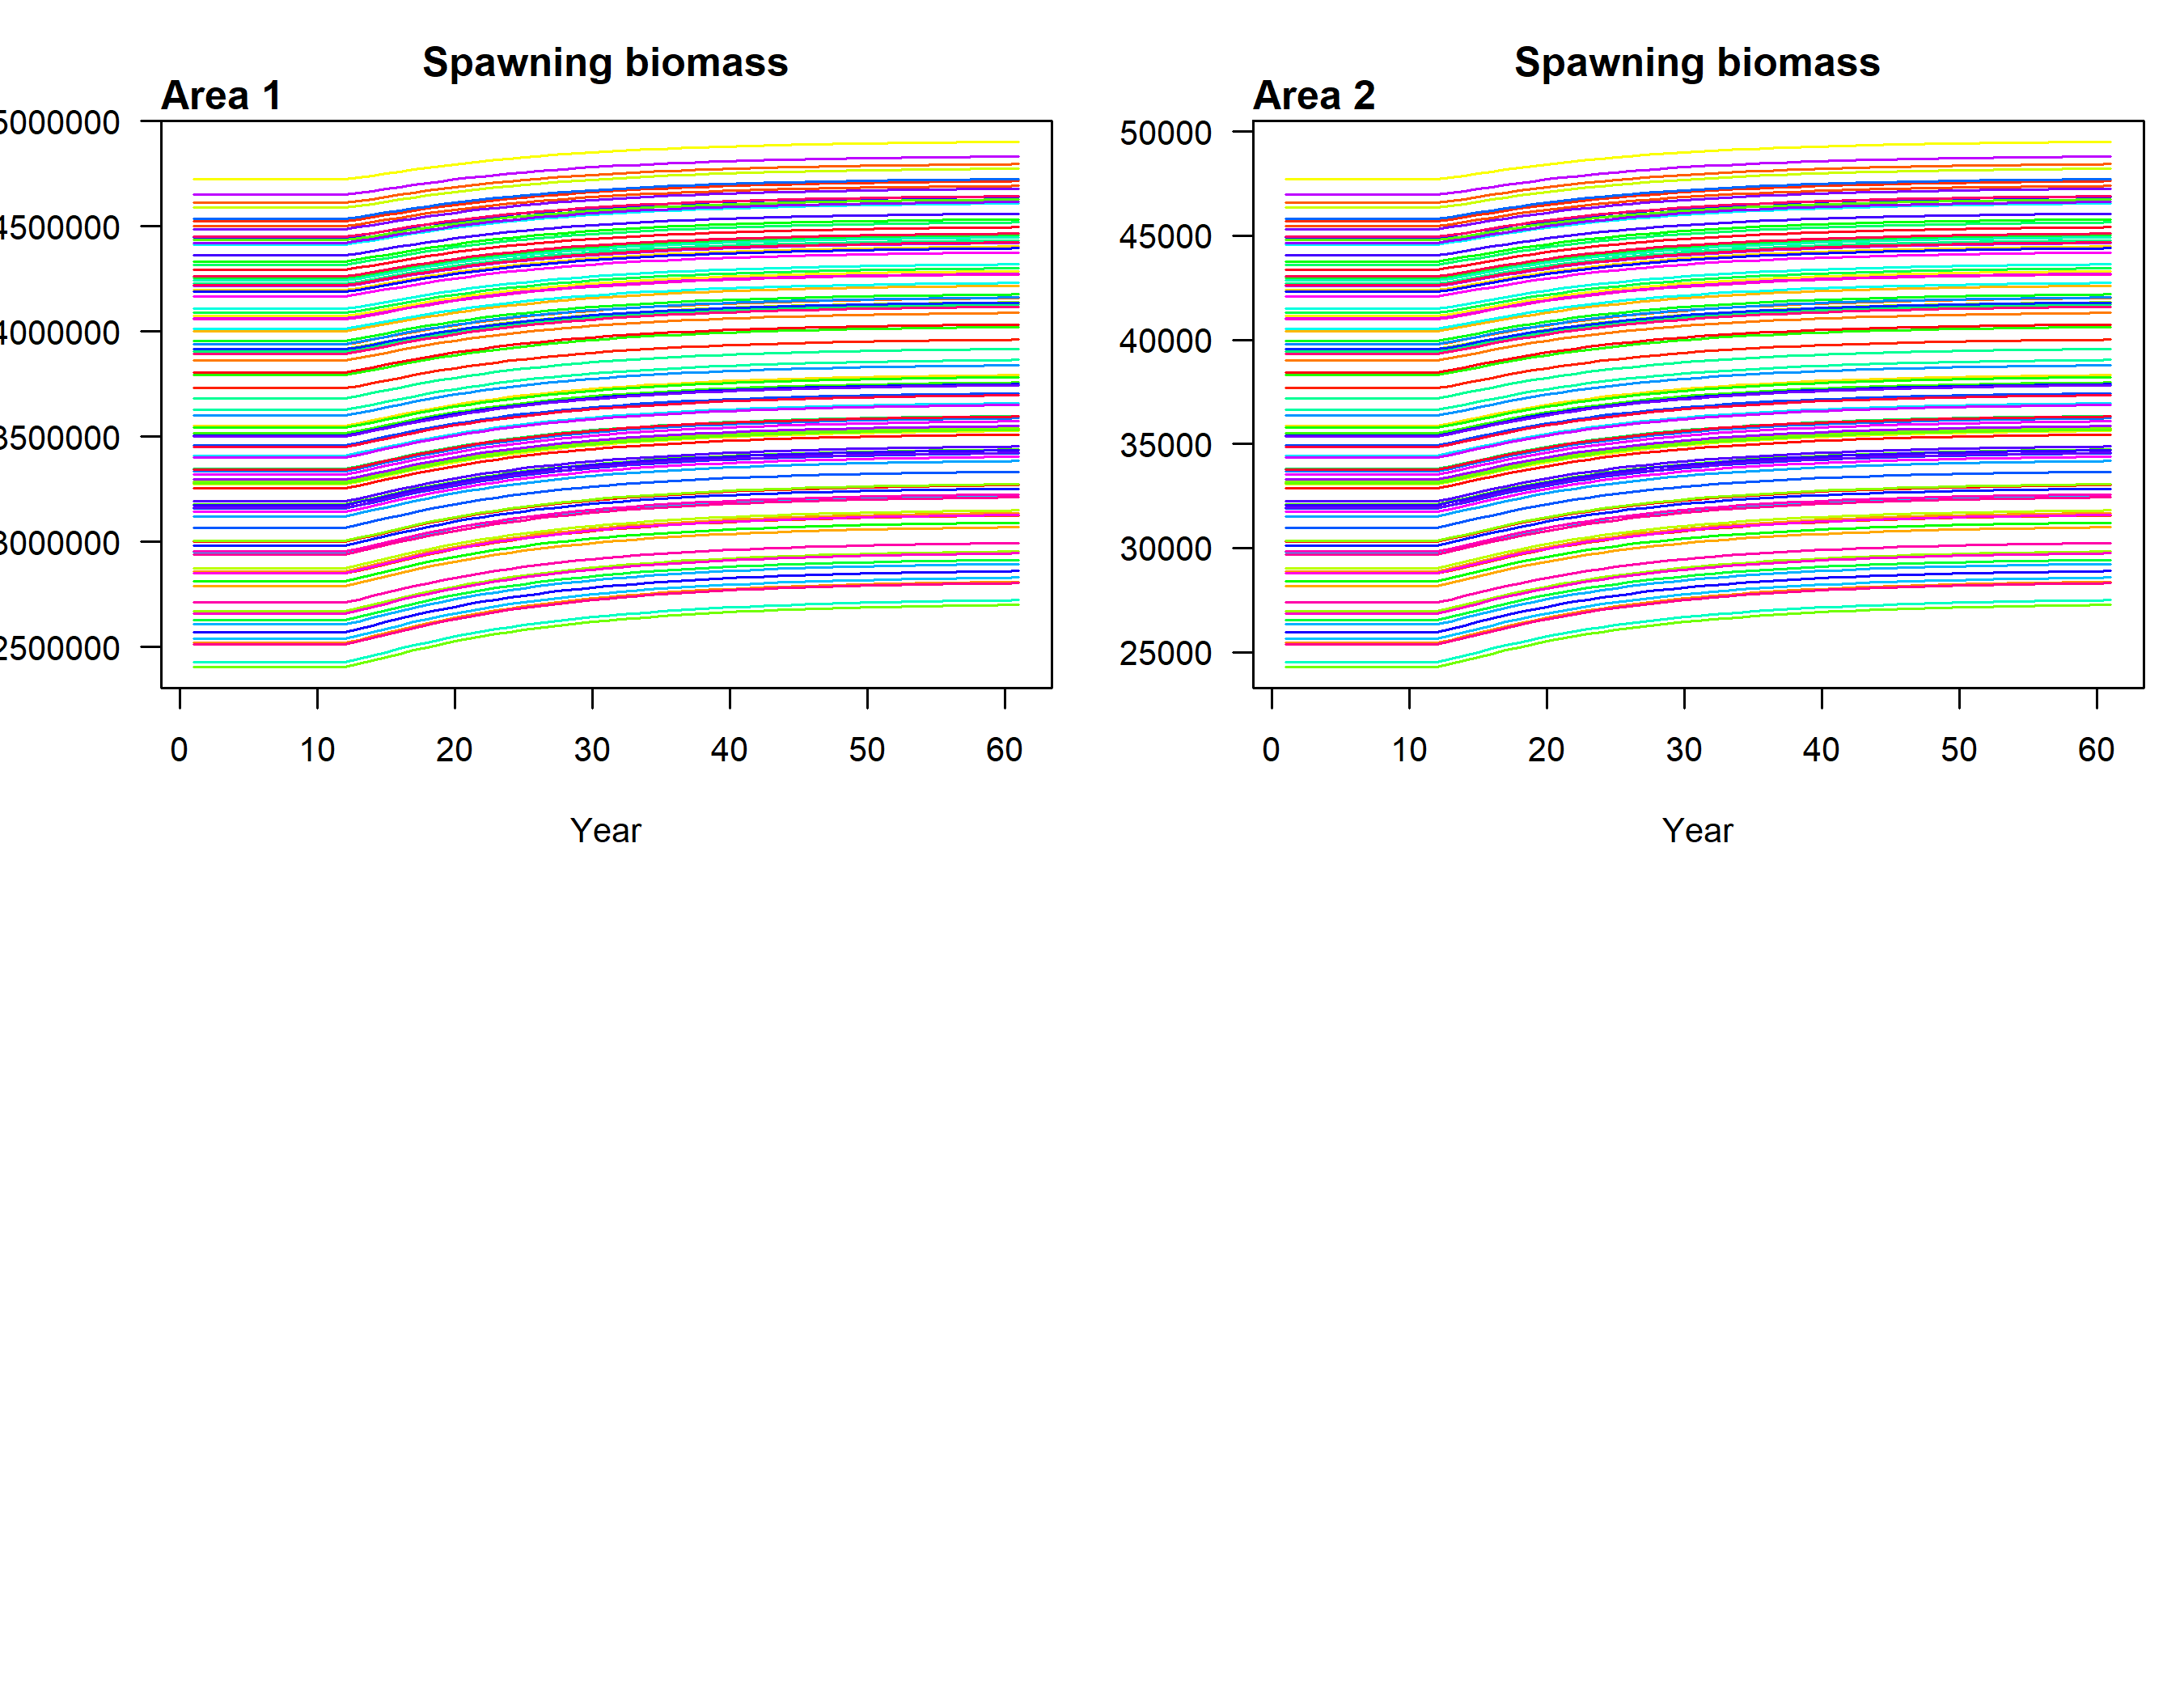
\includegraphics[width=1\linewidth]{data-test/Kole/Higher_option3_SB_Area} \caption{Spawning biomass by area- Higher_option3 }\label{fig:fig-SB-H-opt3}
\end{figure}

\begin{figure}
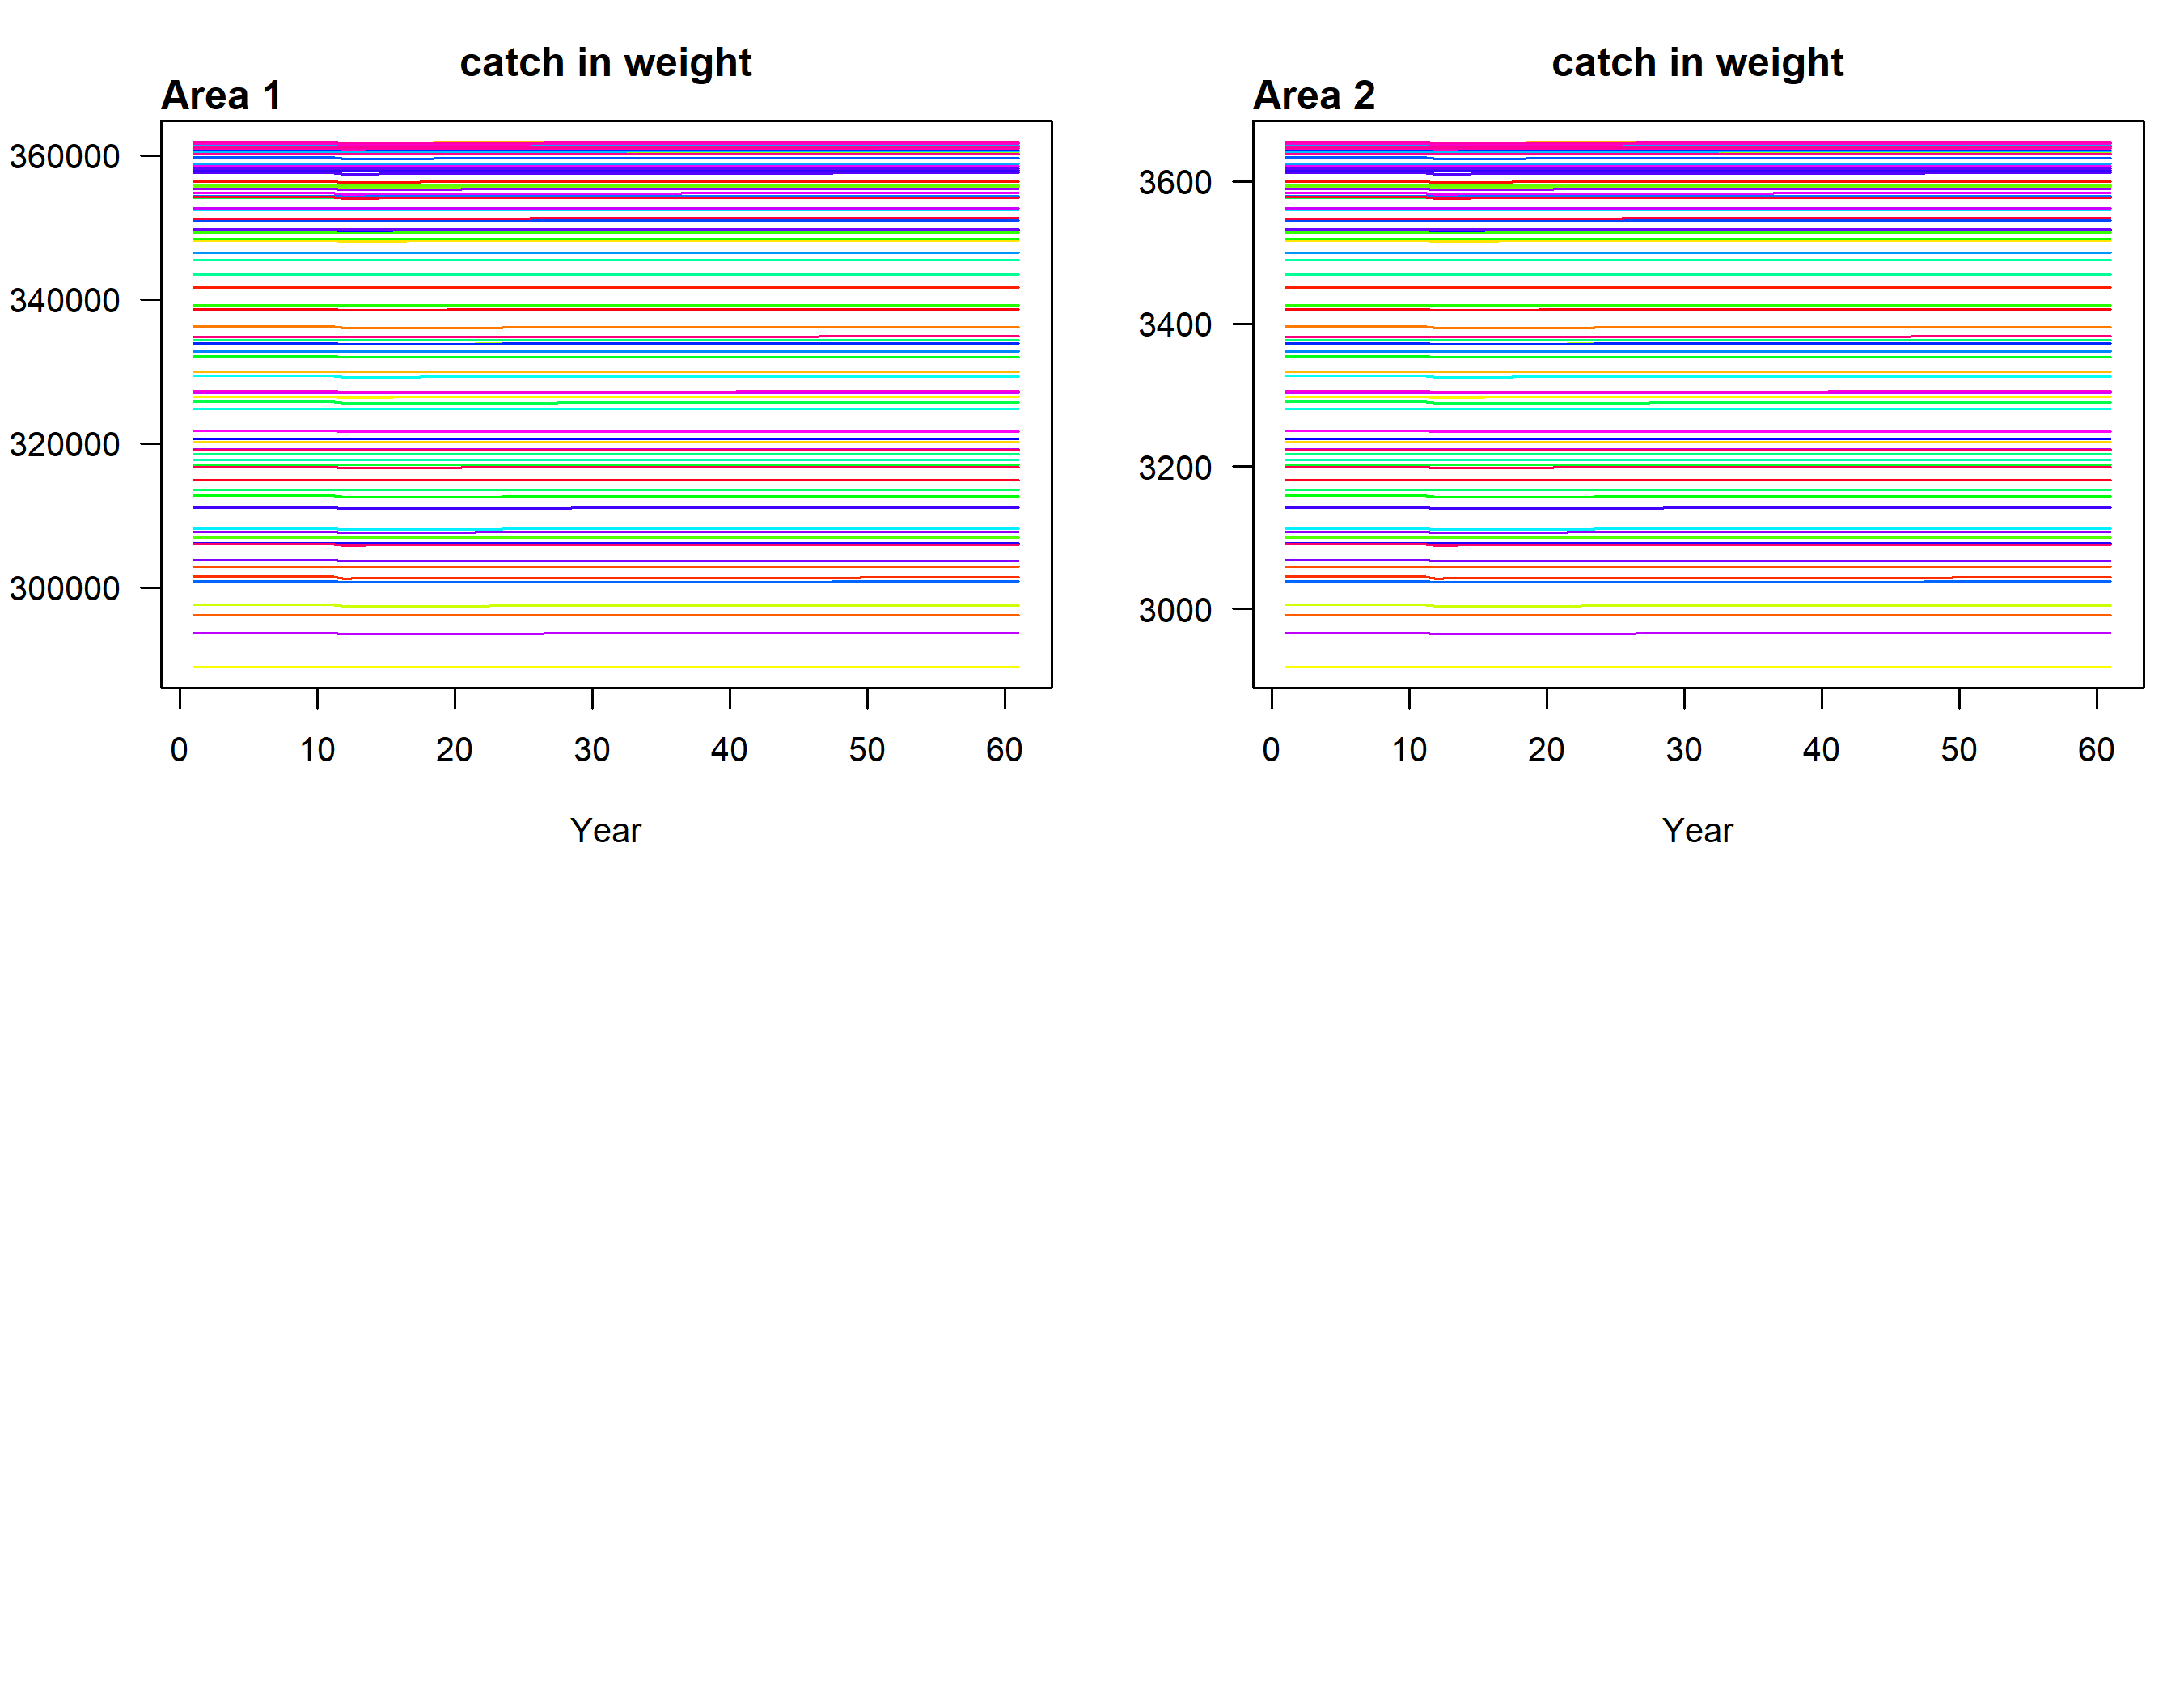
\includegraphics[width=1\linewidth]{data-test/Kole/Higher_option1_catchB_Area} \caption{Catch biomass by area- Higher_option1 }\label{fig:fig-catch-H-opt1}
\end{figure}

\begin{figure}
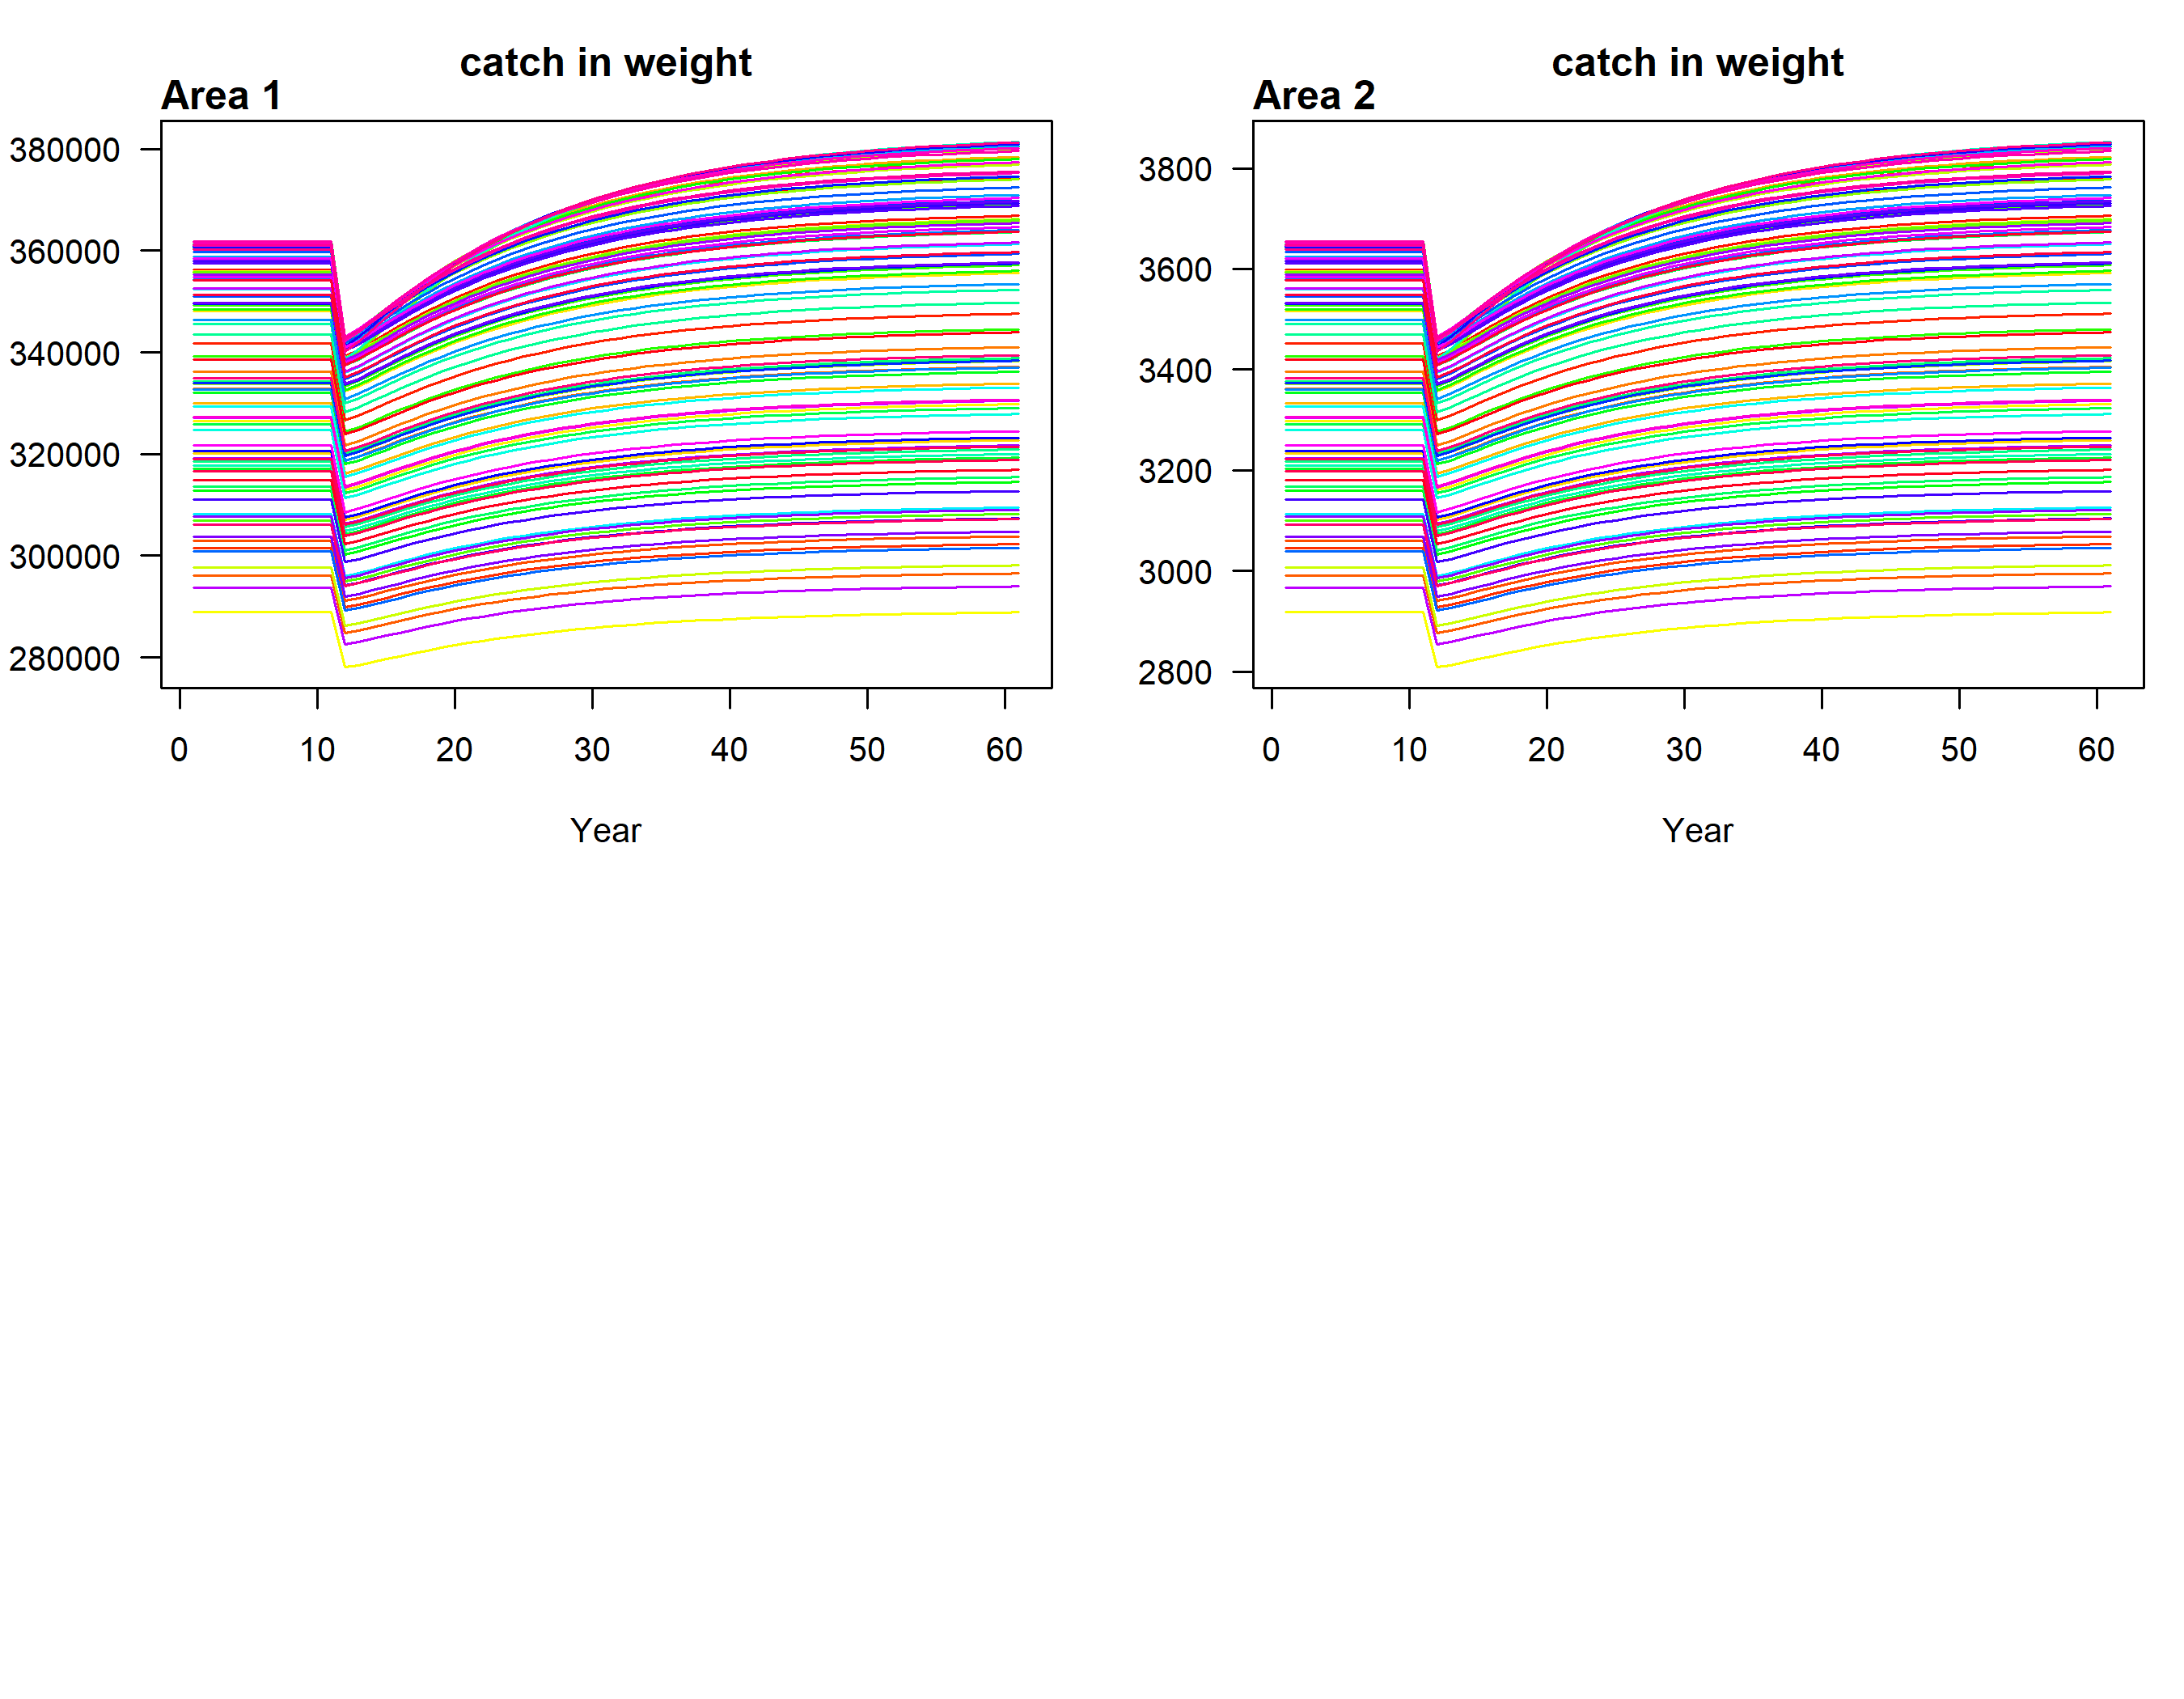
\includegraphics[width=1\linewidth]{data-test/Kole/Higher_option2_catchB_Area} \caption{Catch biomass by area- Higher_option2 }\label{fig:fig-catch-H-opt2}
\end{figure}

\begin{figure}
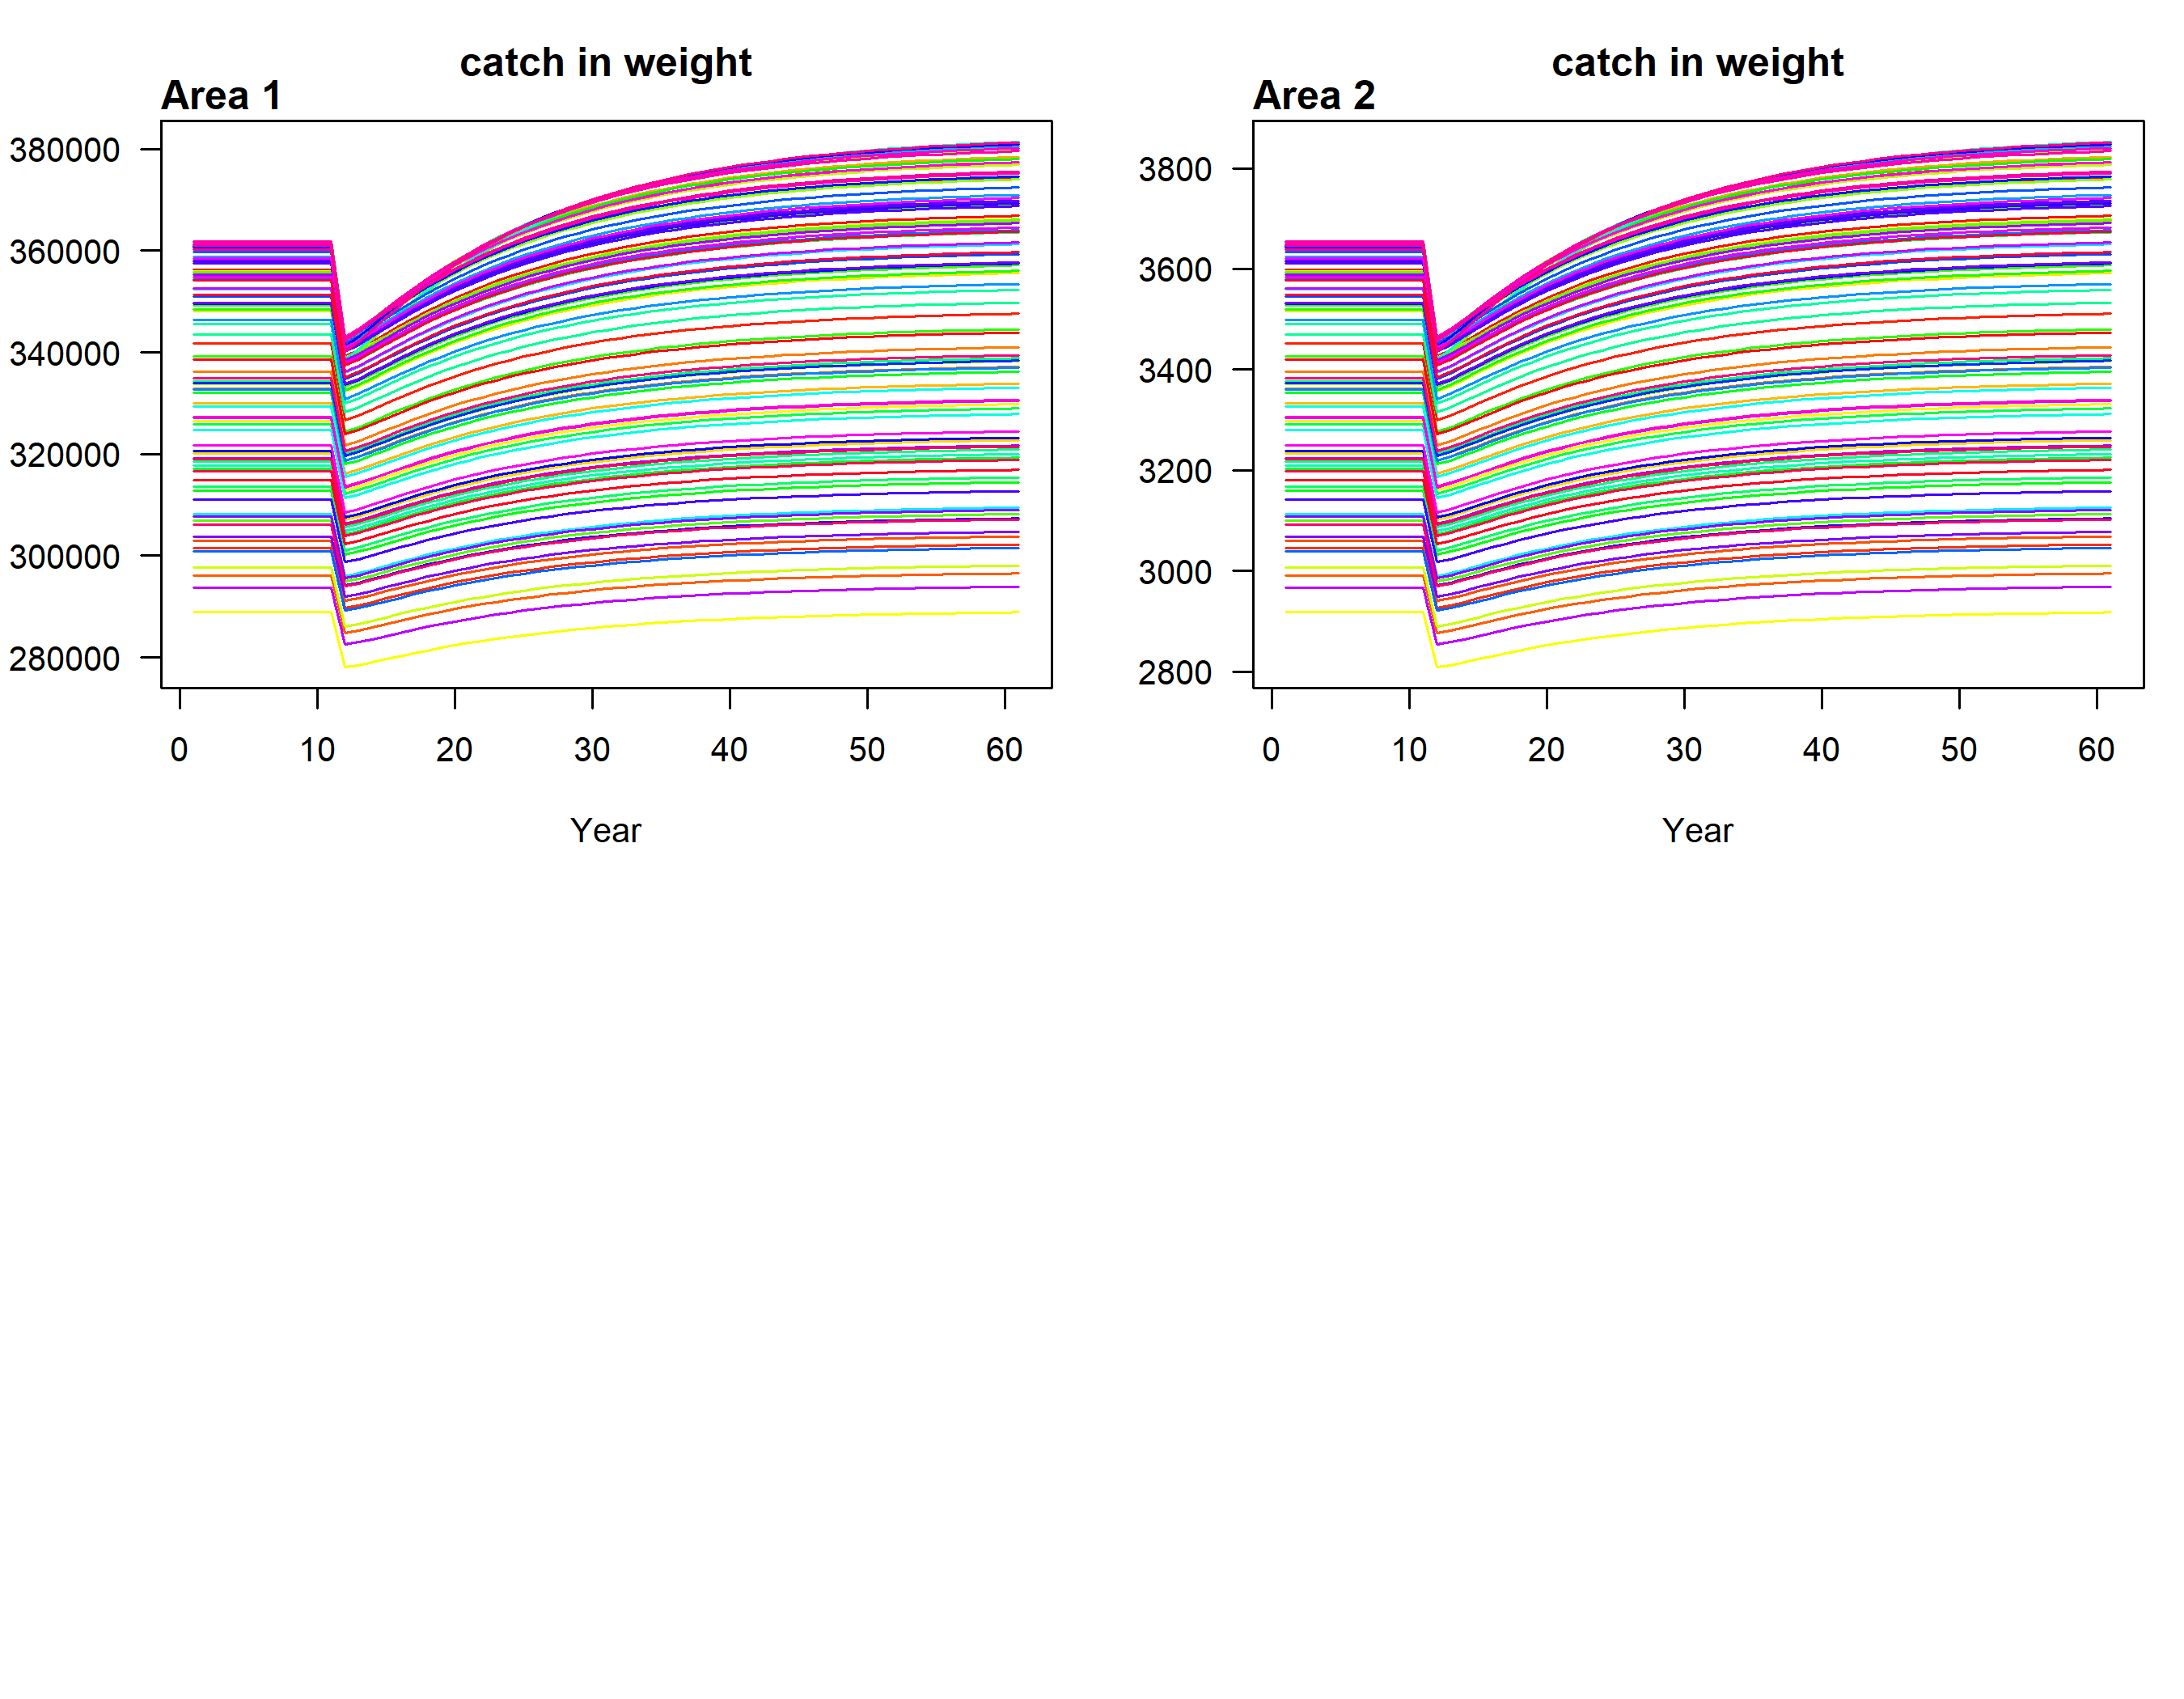
\includegraphics[width=1\linewidth]{data-test/Kole/Higher_option3_catchB_Area} \caption{Catch biomass by area- Higher_option3 }\label{fig:fig-catch-H-opt3}
\end{figure}

\chapter{Mathematical description of the Operating model (OM)}\label{OM}

~~~~An operating model is a mathematical representation of the biology of a fish stock and the fishery that operates on the fish stock. The operating model should also include a sub-model that reflects how the management regulations are implemented and are adhered to in practice \citep{punt_management_2016}.

\section{Population dynamics}\label{population-dynamics}

~~~~The operating model (OM) describes the age-structured population dynamics of a fish population or stock. Population dynamics are specified for a single sex, with dynamics operating on an annual time step, and allowing for migration between multiple areas. Abundance at age, \(a\), at the start of year \(t\), and in area \(i\), \(N_{a,t,i}\) is given by:

\[
N_{0,t,i} = \rho_i R_t, \tag{eq. 1} \label{eq:first}
\]

And,

\[
N_{a+1,t+1,i} = S_{a,t,i} \left(N_{a,t,i}\theta_{i \rightarrow i}+\sum_{j \neq i} N_{a,t,j}\theta_{j \rightarrow i}\right). \tag{eq. 2} \label{eq:second}
\]

Equation \ref{eq:first} is the fraction, \(\rho_i\), of total age-0 recruits, \(R_t\), at the start of the year that are added to area \(i\). In equation \ref{eq:second}, the term in parenthesis describes the fraction of abundance-at-age that does not emigrate from area \(i\), \(\theta_{i \rightarrow i}\), plus the summation of abundance-at-age arriving from all other areas, \(j\), \(\theta_{a,j \rightarrow i}\). In this form, Equation \ref{eq:second} specifies migration to occur at the beginning of the year, followed by survival, \(S_{a,t,i}\), from age \(a\) to age \(a+1\).\\
\strut ~~~~The multi-area model is implemented in matrix form, analogous to a Leslie matrix, as described by \citet{quinn_quantitative_1999}. For brevity, the matrix form is summarized using a two-area example, reflecting the description provided by \citet{quinn_quantitative_1999}, but note that the operating model is generalized as a multi-area model. To account for migration between two areas, \(i\) and \(j\), abundance-at-age in the matrix form is:

\[
\mathbf{N}_{t+1} = \mathbf{P}\mathbf{N}_t, \tag{eq. 3} \label{eq:third}
\]

where \(\mathbf{N}_t\) for ages 0 to maximum age, \(A\), is written:

\[
\mathbf{N}_t =
\begin{pmatrix}
\mathbf{N}_{t,i} \\
\mathbf{N}_{t,j}
\end{pmatrix}
=
\begin{pmatrix}
N_{1,t,i} \\
\vdots \\
N_{A,t,i} \\
N_{1,t,j} \\
\vdots \\
N_{A,t,j}
\end{pmatrix}.
\tag{eq. 4} \label{eq:fourth}
\]

The projection matrix \(\mathbf{P}\) is

\[
\mathbf{P} = \begin{pmatrix}
P_{i,j} & P_{i,j} \\
P_{i,j} & P_{i,j}
\end{pmatrix}, \tag{eq. 5} \label{eq:fifth}
\]

where each element, \(P_{i,j}\), is a matrix that accounts for movement and survival. The matrices, \(P_{i,j}\), are populated as:

\[
P_{i,i} = \begin{pmatrix}
0 & 0 & 0 & 0 & 0 \\
S_{1,t,i}\theta_{1,i\rightarrow i} & 0 & 0 & 0 \\
0 & S_{2,t,i}\theta_{2,i\rightarrow i} & 0 & 0 & 0 \\
0 & 0 & \ddots & 0 & 0 \\
0 & 0 & 0 & S_{A-1,t,i}\theta_{A-1,i\rightarrow i} & S_{A,t,i}\theta_{A,i\rightarrow i}
\end{pmatrix}, \tag{eq. 6} \label{eq:sixth} 
\]

And,

\[
P_{i,j} = \begin{pmatrix}
0 & 0 & 0 & 0 & 0 \\
S_{1,t,i}\theta_{1,j\rightarrow i} & 0 & 0 & 0 \\
0 & S_{2,t,i}\theta_{2,j\rightarrow i} & 0 & 0 & 0 \\
0 & 0 & \ddots & 0 & 0 \\
0 & 0 & 0 & S_{A-1,t,i}\theta_{A-1,j\rightarrow i} & S_{A,t,i}\theta_{A,j\rightarrow i}
\end{pmatrix}. \tag{eq. 7} \label{eq:seventh} 
\]

The operating model specifies a plus group in position (\(A,A\)).\\
\strut ~~~~Total annual recruitment is calculated according to the \citet{beverton_dynamics_1957} stock-recruitment function, which is parameterized using steepness \((h)\):

\[
R_t = \left(\frac{0.8R_0hB_t}{0.2B_0\left(1-h\right) + \left(h-0.2\right)B_t}\right) \exp{\left(d_t - \frac{{\sigma_R}^2}{2}\right)},  \tag{eq. 8} \label{eq:eighth}
\]

where \(B_0\) is unfished reproductive output, \(R_0\) is unfished recruitment, and \(d\) is the annual recruitment deviation, where \(\sigma_R\) is recruitment variability. Annual reproductive output, \(B_t\), is aggregate output (e.g., spawning biomass) for all areas combined, excluding any reproductive contribution of age-0 recruits created at the beginning of the year. Calculated total recruits are distributed to each area in proportion to the area-specific fraction, \(\rho_i\), with \(\sum\rho_i=1\). An overall recruitment deviation signal (e.g., a surrogate for an environmental condition affecting recruitment success) is generated from a normal distribution with mean zero and standard deviation, \(\sigma_R\), (e.g., \(\sigma_R\) = 0.6). Inter-annual autocorrelation in recruitment can be specified, producing 1-year lagged correlation in log-scale recruitment deviations.

\section{Life history}\label{life-history}

~~~~Length is calculated at the start of the year according to the von Bertalanffy growth curve, where \(L_\infty\) is asymptotic length, \(K\) is the growth rate, and parameter \(t_0\):

\[
L_a = L_\infty \left(1- \exp{\left(-K\left(a - t_0\right)\right)}\right). \tag{eq. 9} \label{eq:nineth}
\]

Weight-at-age, \(W_a\), with parameters \(a\) and \(b\) is specified as an exponential function:

\[
W_a=\alpha L_a^\beta. \tag{eq. 10} \label{eq:tenth}
\]

Maturation follows a logistic function with parameters \(L50\) and \(L95\), reflecting the lengths at which 50\% and 95\% of the population are mature, respectively. Optionally, species can be specified as protogynous hermaphroditic species, with proportion of male in the population following an increasing logistic function with parameters \(H50\) and \(H95\), reflecting the lengths at which 50\% and 95\% of the population are male, respectively. For gonochoristic species, a 50:50 sex ratio is assumed at all lengths or ages. Total reproductive output, \(B_t\), is a summation of mature biomass across age classes and areas:

\[
B_t=\sum_{i}\sum_{a}{N_{a,t,i}W_a\mathit{mat}_a{propFemale}_a}, \tag{eq. 11} \label{eq:eleventh}
\]

Where \(propFemale\) is proportion of the population female at age, with a value of 0.5 for all ages for gonochoristic species and values of 1-\(propMale_a\) when sexual transition from female to male is specified.\\
\strut ~~~~Both natural mortality and maximum age can be specified. When maximum age, \(A\), is specified, this quantity is used in constructing abundance matrices. Maximum must be equal to or greater than 2, as this modeling framework is not well suiting to species with very fast life histories. When maximum age is not specified, the age to which 1\% the population survives in an unfished system is used to calculate maximum age, using the formula:

\[
A=\ ceiling\left(-\frac{\log{\left(0.01\right)}}{M}\right) \tag{eq. 12} \label{eq:twelftth}
\]

Uncertainty in life history can be accounted for by specifying parameter ranges, rather than point estimates for most life history parameters. Each iteration will produce a unique set of life history parameters based on independent draws from uniform distributions that correspond to the specified minimum and maximum for each parameter.

\section{Initial conditions}\label{initial-conditions}

~~~~This modeling framework was developed to create historical dynamics of fish stocks that begin (i.e., year 0) in a fished state, meaning that fishing mortality (and consequently fishing effort) are greater than zero in the initial equilibrium year (year 0). Thus, the modeling framework is not suitable for circumstances for initializing the model in an unfished or pre-fishing state. Accordingly, initial depletion should always be less than 1.0. As the state of depletion of each species may be uncertain, initial depletion is implemented as a range of plausible values, producing slightly different values for each iteration. At the beginning of each iteration, initial depletion (i.e., initial spawning biomass relative to unfished spawning biomass) based on a draw from a uniform distribution with a specified minimum and maximum. An alternative formulation is available in that initial `depletion' can instead be specified as initial SPR. Subsequently, the population is initialized as follows. First, equilibrium age-structure is determined for the given depletion level assuming area-specific recruitment fractions, \(\rho_i\), but no movement, resulting in an equilibrium fishing mortality rate and equilibrium abundance scaled relative to the specified \(R_0\). Second, a burn-in period is used to project the population forward for \(A\)x4 years at the estimated equilibrium fishing mortality rate, allowing a stable age distribution between areas to be obtained through migration. Elements that account for uncertainty (initial depletion, life history, selectivity, and annual recruitment deviations) are generated ahead of simulation runs and retained to ensure that each management strategy can be subject to the same sets of stochastic elements, and thus not subject to chance differences in draws from sampling distributions.

\section{Fishery dynamics}\label{fishery-dynamics}

~~~~Survival (\(S\)) consists of natural mortality (\(M\) year\(^{-1}\), fishing mortality (\(F\) year\(^{-1}\)):

\[
S_{a,t,i}=exp{\left(-M-{\mathit{Removal}}_aF_{t,i}\right)}, \tag{eq. 13} \label{eq:thirteenth} 
\]

where \(Removal\) is a component of fishery selectivity and is covered in a subsequent section.\\
Landings in numbers (\(C^{N}\) is:

\[
C_{a,t,i}^N=\frac{{\mathit{Keep}}_aF_{t,i}}{\left(M_s+{\mathit{Removal}}_aF_{t,i}\right)}\left(1-S_{a,t,i}\right)N_{a,t,i}, \tag{eq. 14} \label{eq:fourteenth}
\]

and \(keep\) is a component of fishery selectivity. Landings in weight (\(C^B\)) is:

\[
C_{a,t,i}^B=C_{a,t,i}^NW_a \tag{eq. 15} \label{eq:fifteenth}
\]

Fishery selectivity is defined as follows. Vulnerability to the fishing gear, \(Vul\), is currently includes lognormal selectivity (parameterized for gillnet parameter inputs) and logistic selectivity, with input parameters \(SL50\) and \(SL95\), reflecting the lengths at which 50\% and 95\% of the population are mature vulnerable to the gear, respectively. Retention, \(Ret\), can be specified as `full', resulting in full retention across all vulnerable size classes, `logistic' or `slot limit'. Additionally, the maximum level of retention (e.g., a quantity between 0 and 1) can be specified for any of the above stated retention types. Finally, a discard mortality proportion, \(D\), (e.g.~quantity between 0 and 1) can be specified to affect the fate of discards. These inputs are used in calculating the following components of fishery selectivity.

\(Keep\) - \emph{the resulting probability of being landed}
\[
Keep_a=Vul_aRet_a \tag{eq. 16} \label{eq:sixteenth}
\]

\(Dead\,discards\) - \emph{deaths resulting from vulnerable abundance that is not retained}
\[
Dead\,discards_a=Vul_a(1-Ret_a)D \tag{eq. 17} \label{eq:seventeenth}
\]

\(Total\,removals\) -- \emph{probability of removal from the population via landing or discard}
\[
Removal_a=Vul_a(Ret_a+(1-Ret_a)D) \tag{eq. 18} \label{eq:eighteenth}
\]

Uncertainty in vulnerability and retention can be accounted for by specifying parameter ranges, rather than point estimates. Each iteration will produce a unique selectivity and/or retention characteristics based on independent draws from uniform distributions that correspond to the specified minimum and maximum for each parameter.

\section{Observation and monitoring}\label{observation-and-monitoring}

~~~~Depending on the specific application of the model, an observation model may be required. This requirement is driven by whether a harvest control rule is used in decision-making. That is, whether some form of data collection will inform year-to-year adjustments in a total allowable catch or total fishery effort. If so, then simulation of the data observation processes (including imperfect observation) is required. Observation models tend to be tailored to the type of data collection program that is in place. This component should be developed as needed for each unique application.

\section{Growth-type group}\label{growth-type-group}

To account for individual variation in growth trajectories, the population is divided into growth-type groups (GTGs) or cohorts \citep[\citet{pine_iii_curious_2015}, \citet{hordyk_simple_2016}]{walters_fisheries_2004}. GTGs describe the variation in growth of a fish population through the creation of \(G\) groups and with dimensions indexed \(g=1,2…G\). Each group differs in terms of its \(L_\infty\). Given a mean value, \(\bar{L}_\infty\) and a standard deviation (calculated as a coefficient of variation, \(CV_L\) times \(\bar{L}_\infty\)), the range of \(L_\infty\) ± two standard deviations is divided into \(G\) equal increments. A default value of \(CV_L\) = 0.1 and \(G\) = 13 groups, results in \(g\) = 7 representing \(\bar{L}_\infty\). Cohort size assigned to each group is determined by distributing a fraction of annual recruits in each group, \(p\), where \(\sum{p}=1\). Vector \(p\) is determined as proportional to the \(G\) increments in \(L_\infty\) along the probability density function of a normal distribution with mean \(\bar{L}_\infty\) and variance \(\left(CV_L{\bar{L}}_\infty\right)^2\). Functionality is also included such that if \(G\) = 1, the model collapses to a simpler age-based model.

\chapter{Customized Management Procedures (MPs)}\label{customized-management-procedures-mps}

Adding customized MPs in this section

\section{MP 1}\label{mp-1}

add text

\section{MP 2}\label{mp-2}

add text

\chapter{The Closed Loop Simulation}\label{the-closed-loop-simulation}

This chapter explains\ldots..

\chapter{Exploring the Simulation Outputs}\label{exploring-the-simulation-outputs}

This shows outputs of the simulation

\chapter{Examples}\label{examples}

\section{Honeycomb grouper example}\label{honeycomb-grouper-example}

This example illustrates a model with four areas and a suite of management options, including size limits, effort reductions (such as seasonal closures or time-day closures), and rotational spatial closures. All simulations are conducted under the assumption that fishing effort is reallocated from closed areas to open areas, rather than being removed from the fishery.

See Section \ref{OM-pop} for details on how to populate the Operating Model.

\subsection{Populationg the life history}\label{populationg-the-life-history}

\begin{Shaded}
\begin{Highlighting}[]
\NormalTok{LifeHistoryObj }\OtherTok{\textless{}{-}} \FunctionTok{new}\NormalTok{(}\StringTok{"LifeHistory"}\NormalTok{)}
\NormalTok{LifeHistoryObj}\SpecialCharTok{@}\NormalTok{title}\OtherTok{\textless{}{-}}\StringTok{"Honeycomb grouper"}
\NormalTok{LifeHistoryObj}\SpecialCharTok{@}\NormalTok{speciesName}\OtherTok{\textless{}{-}}\StringTok{"EpinephelusMerra"}
\NormalTok{LifeHistoryObj}\SpecialCharTok{@}\NormalTok{shortDescription}\OtherTok{\textless{}{-}}\StringTok{"example multiple areas"}
\NormalTok{LifeHistoryObj}\SpecialCharTok{@}\NormalTok{Linf}\OtherTok{\textless{}{-}}\FloatTok{24.4}
\NormalTok{LifeHistoryObj}\SpecialCharTok{@}\NormalTok{K}\OtherTok{\textless{}{-}}\FloatTok{0.2}
\NormalTok{LifeHistoryObj}\SpecialCharTok{@}\NormalTok{t0}\OtherTok{\textless{}{-}} \DecValTok{0}
\NormalTok{LifeHistoryObj}\SpecialCharTok{@}\NormalTok{L50}\OtherTok{\textless{}{-}}\FloatTok{14.1}
\NormalTok{LifeHistoryObj}\SpecialCharTok{@}\NormalTok{L95delta}\OtherTok{\textless{}{-}}\FloatTok{2.1}
\NormalTok{LifeHistoryObj}\SpecialCharTok{@}\NormalTok{M}\OtherTok{\textless{}{-}}\FloatTok{0.29}
\NormalTok{LifeHistoryObj}\SpecialCharTok{@}\NormalTok{L\_type}\OtherTok{\textless{}{-}}\StringTok{"FL"}
\NormalTok{LifeHistoryObj}\SpecialCharTok{@}\NormalTok{L\_units}\OtherTok{\textless{}{-}}\StringTok{"cm"}
\NormalTok{LifeHistoryObj}\SpecialCharTok{@}\NormalTok{LW\_A}\OtherTok{\textless{}{-}}\FloatTok{0.016}
\NormalTok{LifeHistoryObj}\SpecialCharTok{@}\NormalTok{LW\_B}\OtherTok{\textless{}{-}}\FloatTok{2.966}
\NormalTok{LifeHistoryObj}\SpecialCharTok{@}\NormalTok{Walpha\_units}\OtherTok{\textless{}{-}}\StringTok{"g"}
\NormalTok{LifeHistoryObj}\SpecialCharTok{@}\NormalTok{Steep}\OtherTok{\textless{}{-}}\FloatTok{0.69}
\NormalTok{LifeHistoryObj}\SpecialCharTok{@}\NormalTok{recSD}\OtherTok{\textless{}{-}}\FloatTok{0.6}
\NormalTok{LifeHistoryObj}\SpecialCharTok{@}\NormalTok{recRho}\OtherTok{\textless{}{-}}\DecValTok{0}
\NormalTok{LifeHistoryObj}\SpecialCharTok{@}\NormalTok{isHermaph}\OtherTok{\textless{}{-}}\ConstantTok{FALSE}
\NormalTok{LifeHistoryObj}\SpecialCharTok{@}\NormalTok{R0}\OtherTok{\textless{}{-}}\DecValTok{10000}
\end{Highlighting}
\end{Shaded}

\subsection{Populating the fishery history}\label{populating-the-fishery-history}

\begin{Shaded}
\begin{Highlighting}[]
\NormalTok{HistFisheryObj}\OtherTok{\textless{}{-}}\FunctionTok{new}\NormalTok{(}\StringTok{"Fishery"}\NormalTok{)}
\NormalTok{HistFisheryObj}\SpecialCharTok{@}\NormalTok{title}\OtherTok{\textless{}{-}}\StringTok{"Test"}
\NormalTok{HistFisheryObj}\SpecialCharTok{@}\NormalTok{vulType}\OtherTok{\textless{}{-}}\StringTok{"logistic"}
\NormalTok{HistFisheryObj}\SpecialCharTok{@}\NormalTok{vulParams}\OtherTok{\textless{}{-}}\FunctionTok{c}\NormalTok{(}\DecValTok{19}\NormalTok{, }\FloatTok{0.9}\NormalTok{)}
\NormalTok{HistFisheryObj}\SpecialCharTok{@}\NormalTok{retType}\OtherTok{\textless{}{-}}\StringTok{"full"}
\NormalTok{HistFisheryObj}\SpecialCharTok{@}\NormalTok{retMax }\OtherTok{\textless{}{-}} \DecValTok{1}
\NormalTok{HistFisheryObj}\SpecialCharTok{@}\NormalTok{Dmort }\OtherTok{\textless{}{-}} \DecValTok{0}
\end{Highlighting}
\end{Shaded}

\subsection{Populating the time and area parameters}\label{populating-the-time-and-area-parameters}

\begin{Shaded}
\begin{Highlighting}[]
\CommentTok{\# I want to run the low movement scenario}
\NormalTok{TimeAreaObj}\OtherTok{\textless{}{-}}\FunctionTok{new}\NormalTok{(}\StringTok{"TimeArea"}\NormalTok{)}
\NormalTok{TimeAreaObj}\SpecialCharTok{@}\NormalTok{title }\OtherTok{=} \StringTok{"Test"}
\NormalTok{TimeAreaObj}\SpecialCharTok{@}\NormalTok{gtg }\OtherTok{=} \DecValTok{13}
\NormalTok{TimeAreaObj}\SpecialCharTok{@}\NormalTok{areas }\OtherTok{=} \DecValTok{4}
\NormalTok{TimeAreaObj}\SpecialCharTok{@}\NormalTok{recArea }\OtherTok{=} \FunctionTok{c}\NormalTok{(}\FloatTok{0.067}\NormalTok{, }\FloatTok{0.067}\NormalTok{,}\FloatTok{0.067}\NormalTok{,}\FloatTok{0.8}\NormalTok{)}\CommentTok{\#rec pars excel?}
\NormalTok{TimeAreaObj}\SpecialCharTok{@}\NormalTok{iterations }\OtherTok{=} \DecValTok{100}
\NormalTok{TimeAreaObj}\SpecialCharTok{@}\NormalTok{historicalYears }\OtherTok{=} \DecValTok{50}
\NormalTok{TimeAreaObj}\SpecialCharTok{@}\NormalTok{historicalBio }\OtherTok{=} \FloatTok{0.5}
\NormalTok{TimeAreaObj}\SpecialCharTok{@}\NormalTok{historicalBioType }\OtherTok{=} \StringTok{"relB"}
\NormalTok{TimeAreaObj}\SpecialCharTok{@}\NormalTok{move }\OtherTok{\textless{}{-}} \FunctionTok{matrix}\NormalTok{(}\FunctionTok{c}\NormalTok{(}
  \FloatTok{0.9}\NormalTok{, }\FloatTok{0.05}\NormalTok{, }\FloatTok{0.05}\NormalTok{, }\DecValTok{0}\NormalTok{,}
  \FloatTok{0.05}\NormalTok{, }\FloatTok{0.9}\NormalTok{, }\FloatTok{0.05}\NormalTok{, }\DecValTok{0}\NormalTok{,}
  \FloatTok{0.05}\NormalTok{, }\FloatTok{0.05}\NormalTok{, }\FloatTok{0.9}\NormalTok{, }\DecValTok{0}\NormalTok{,}
  \DecValTok{0}\NormalTok{, }\DecValTok{0}\NormalTok{, }\DecValTok{0}\NormalTok{, }\DecValTok{0}\NormalTok{), }\AttributeTok{nrow=}\DecValTok{4}\NormalTok{, }\AttributeTok{ncol=}\DecValTok{4}\NormalTok{, }\AttributeTok{byrow=}\ConstantTok{TRUE}\NormalTok{) }\CommentTok{\#move pars excel?}
\NormalTok{TimeAreaObj}\SpecialCharTok{@}\NormalTok{historicalEffort}\OtherTok{\textless{}{-}}\FunctionTok{matrix}\NormalTok{(}\DecValTok{1}\SpecialCharTok{:}\DecValTok{1}\NormalTok{, }\AttributeTok{nrow =} \DecValTok{50}\NormalTok{, }\AttributeTok{ncol =} \DecValTok{4}\NormalTok{, }\AttributeTok{byrow =} \ConstantTok{FALSE}\NormalTok{) }\CommentTok{\#excel time{-}area base {-} hist effort row 1 \textgreater{} effort pars row 1?}
\end{Highlighting}
\end{Shaded}

\subsection{Exploring the paramaterization of the OM so far}\label{exploring-the-paramaterization-of-the-om-so-far}

\begin{Shaded}
\begin{Highlighting}[]
\CommentTok{\#To simply display to the console}
\NormalTok{lhOut}\OtherTok{\textless{}{-}}\FunctionTok{LHwrapper}\NormalTok{(LifeHistoryObj, TimeAreaObj, }\AttributeTok{doPlot =} \ConstantTok{TRUE}\NormalTok{)}
\end{Highlighting}
\end{Shaded}

\begin{figure}
\centering
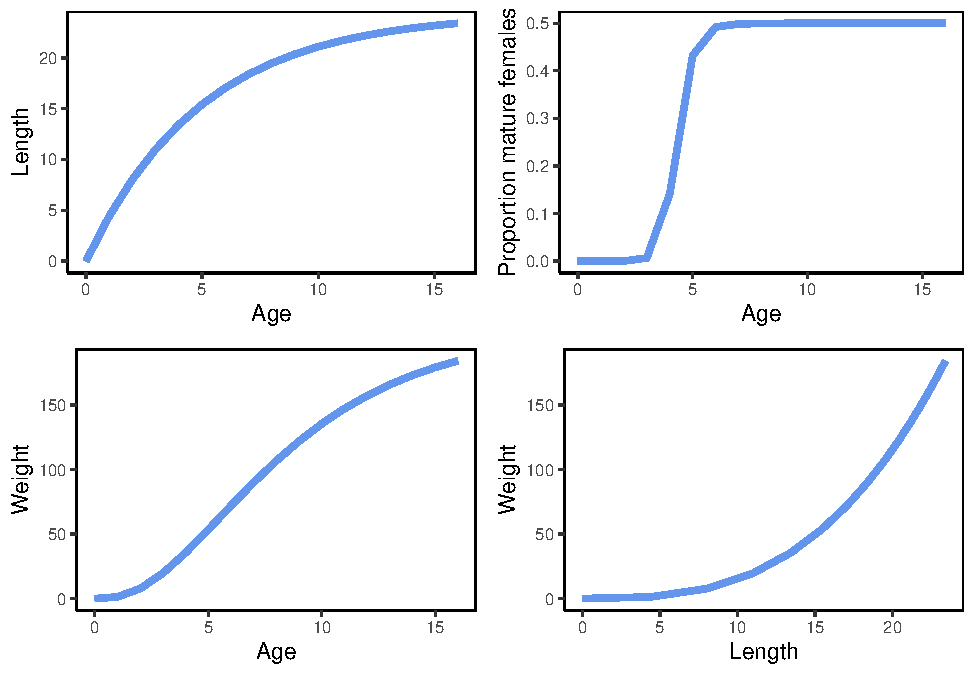
\includegraphics{_main_files/figure-latex/lhgrouper-1.pdf}
\caption{\label{fig:lhgrouper}Life history schedules of honeycomb grouper.}
\end{figure}

\begin{Shaded}
\begin{Highlighting}[]
\CommentTok{\#To return life history details}
\NormalTok{lhOut}
\end{Highlighting}
\end{Shaded}

\begin{Shaded}
\begin{Highlighting}[]
\NormalTok{selOut}\OtherTok{\textless{}{-}}\FunctionTok{selWrapper}\NormalTok{(}\AttributeTok{lh =}\NormalTok{ lhOut, TimeAreaObj, }\AttributeTok{FisheryObj =}\NormalTok{ HistFisheryObj, }\AttributeTok{doPlot =} \ConstantTok{TRUE}\NormalTok{)}
\end{Highlighting}
\end{Shaded}

\begin{figure}
\centering
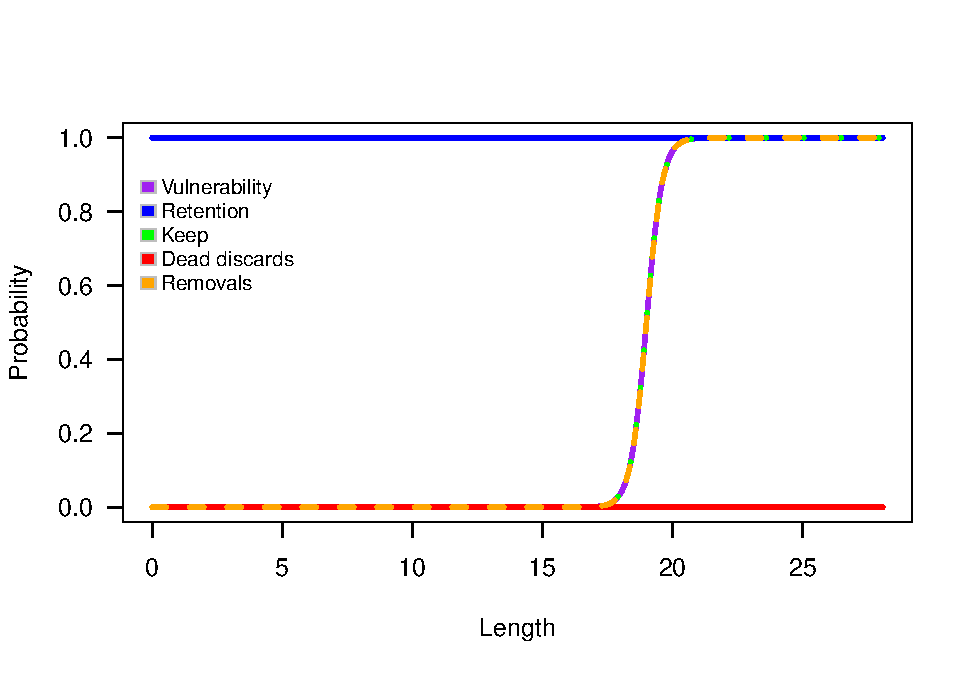
\includegraphics{_main_files/figure-latex/selgrouper-1.pdf}
\caption{\label{fig:selgrouper}Logistic selectivity function.}
\end{figure}

\subsection{Including stochasticity}\label{including-stochasticity}

\begin{Shaded}
\begin{Highlighting}[]
\NormalTok{StochasticObj}\OtherTok{\textless{}{-}}\FunctionTok{new}\NormalTok{(}\StringTok{"Stochastic"}\NormalTok{)}
\NormalTok{StochasticObj}\SpecialCharTok{@}\NormalTok{historicalBio }\OtherTok{=} \FunctionTok{c}\NormalTok{(}\FloatTok{0.2}\NormalTok{, }\FloatTok{0.6}\NormalTok{)}
\NormalTok{StochasticObj}\SpecialCharTok{@}\NormalTok{Linf}\OtherTok{=}\FunctionTok{c}\NormalTok{(}\FloatTok{24.4}\NormalTok{, }\FloatTok{29.8}\NormalTok{)}
\NormalTok{StochasticObj}\SpecialCharTok{@}\NormalTok{K}\OtherTok{=}\FunctionTok{c}\NormalTok{(}\FloatTok{0.2}\NormalTok{, }\FloatTok{0.97}\NormalTok{)}
\NormalTok{StochasticObj}\SpecialCharTok{@}\NormalTok{L50}\OtherTok{=}\FunctionTok{c}\NormalTok{(}\FloatTok{14.1}\NormalTok{, }\FloatTok{16.8}\NormalTok{)}
\NormalTok{StochasticObj}\SpecialCharTok{@}\NormalTok{L95delta}\OtherTok{=}\FunctionTok{c}\NormalTok{(}\FloatTok{2.1}\NormalTok{, }\FloatTok{2.5}\NormalTok{)}
\NormalTok{StochasticObj}\SpecialCharTok{@}\NormalTok{M}\OtherTok{=}\FunctionTok{c}\NormalTok{(}\FloatTok{0.29}\NormalTok{, }\FloatTok{0.43}\NormalTok{)}
\NormalTok{StochasticObj}\SpecialCharTok{@}\NormalTok{Steep}\OtherTok{=}\FunctionTok{c}\NormalTok{(}\FloatTok{0.69}\NormalTok{, }\FloatTok{0.84}\NormalTok{)}
\NormalTok{StochasticObj}\SpecialCharTok{@}\NormalTok{histFisheryVul}\OtherTok{=}\FunctionTok{matrix}\NormalTok{(}\FunctionTok{c}\NormalTok{(}\FloatTok{18.05}\NormalTok{,}\FloatTok{19.95}\NormalTok{,}\FloatTok{0.86}\NormalTok{,}\FloatTok{0.95}\NormalTok{), }\AttributeTok{nrow=}\DecValTok{2}\NormalTok{, }\AttributeTok{ncol=}\DecValTok{2}\NormalTok{,}\AttributeTok{byrow=}\ConstantTok{FALSE}\NormalTok{)  }\CommentTok{\#ask bill {-} stochastic base excel says 1{-} I took sel\_uncert (excel) pars}
\NormalTok{StochasticObj}\SpecialCharTok{@}\NormalTok{sameFisheryVul}\OtherTok{=}\ConstantTok{TRUE}
\end{Highlighting}
\end{Shaded}

\subsection{Fishery projections}\label{fishery-projections-1}

\begin{Shaded}
\begin{Highlighting}[]
\NormalTok{ProFisheryObj}\OtherTok{\textless{}{-}}\FunctionTok{new}\NormalTok{(}\StringTok{"Fishery"}\NormalTok{)}
\NormalTok{ProFisheryObj}\SpecialCharTok{@}\NormalTok{title}\OtherTok{\textless{}{-}}\StringTok{"Test"}
\NormalTok{ProFisheryObj}\SpecialCharTok{@}\NormalTok{vulType}\OtherTok{\textless{}{-}}\StringTok{"logistic"}
\NormalTok{ProFisheryObj}\SpecialCharTok{@}\NormalTok{vulParams}\OtherTok{\textless{}{-}}\FunctionTok{c}\NormalTok{(}\DecValTok{19}\NormalTok{, }\FloatTok{0.9}\NormalTok{) }\CommentTok{\# excel fishery{-}base row3 (is proj?)}
\NormalTok{ProFisheryObj}\SpecialCharTok{@}\NormalTok{retType}\OtherTok{\textless{}{-}}\StringTok{"logistic"}
\NormalTok{ProFisheryObj}\SpecialCharTok{@}\NormalTok{retParams }\OtherTok{\textless{}{-}} \FunctionTok{c}\NormalTok{(}\DecValTok{22}\NormalTok{, }\FloatTok{0.1}\NormalTok{)}\CommentTok{\#excel fishery{-}base row3 (is proj?)}
\NormalTok{ProFisheryObj}\SpecialCharTok{@}\NormalTok{retMax }\OtherTok{\textless{}{-}} \DecValTok{1}
\NormalTok{ProFisheryObj}\SpecialCharTok{@}\NormalTok{Dmort }\OtherTok{\textless{}{-}} \DecValTok{0}
\end{Highlighting}
\end{Shaded}

\subsection{The management strategy}\label{the-management-strategy-1}

Trying to figure out how to implement the 25\% effort reduction?

\begin{Shaded}
\begin{Highlighting}[]
\NormalTok{StrategyObj}\OtherTok{\textless{}{-}}\FunctionTok{new}\NormalTok{(}\StringTok{"Strategy"}\NormalTok{)}
\NormalTok{StrategyObj}\SpecialCharTok{@}\NormalTok{projectionYears }\OtherTok{\textless{}{-}} \DecValTok{50}
\NormalTok{StrategyObj}\SpecialCharTok{@}\NormalTok{projectionName}\OtherTok{\textless{}{-}}\StringTok{"projectionStrategy"}
\CommentTok{\# I took effort from row 3 corresponding to strategy 25\% red}
\NormalTok{eff\_vector}\OtherTok{=}\FunctionTok{scan}\NormalTok{(}\AttributeTok{text=}\NormalTok{(}\StringTok{"0    0   0   0   1.125   1.125   1.125   1.125   1.125   1.125   1.125   1.125   1.125   1.125   1.125   1.125   1.125   1.125   1.125   1.125   1.125   1.125   1.125   1.125   1.125   1.125   1.125   1.125   1.125   1.125   1.125   1.125   1.125   1.125   1.125   1.125   1.125   1.125   1.125   1.125   1.125   1.125   1.125   1.125   1.125   1.125   1.125   1.125   1.125   1.125   0   0   0   0   0   0   0   0   0   0   0   0   0   0   0   0   0   0   0   0   0   0   0   0   0   0   0   0   0   0   0   0   0   0   0   0   0   0   0   0   0   0   0   0   0   0   0   0   0   0   0   0   0   0   1.125   1.125   1.125   1.125   1.125   1.125   1.125   1.125   1.125   1.125   1.125   1.125   1.125   1.125   1.125   1.125   1.125   1.125   1.125   1.125   1.125   1.125   1.125   1.125   1.125   1.125   1.125   1.125   1.125   1.125   1.125   1.125   1.125   1.125   1.125   1.125   1.125   1.125   1.125   1.125   1.125   1.125   1.125   1.125   1.125   1.125   1   1   1   1   1   1   1   1   1   1   1   1   1   1   1   1   1   1   1   1   1   1   1   1   1   1   1   1   1   1   1   1   1   1   1   1   1   1   1   1   1   1   1   1   1   1   1   1   1   1"}\NormalTok{))}

\NormalTok{StrategyObj}\SpecialCharTok{@}\NormalTok{projectionParams}\OtherTok{\textless{}{-}}\FunctionTok{list}\NormalTok{(}\AttributeTok{bag =} \FunctionTok{c}\NormalTok{(}\SpecialCharTok{{-}}\DecValTok{99}  \SpecialCharTok{{-}}\DecValTok{99} \SpecialCharTok{{-}}\DecValTok{99} \SpecialCharTok{{-}}\DecValTok{99}
\NormalTok{), }\AttributeTok{effort =} \FunctionTok{matrix}\NormalTok{(eff\_vector, }\AttributeTok{nrow=}\DecValTok{50}\NormalTok{, }\AttributeTok{ncol=}\DecValTok{4}\NormalTok{, }\AttributeTok{byrow =} \ConstantTok{FALSE}\NormalTok{), }\AttributeTok{CPUE =} \FunctionTok{c}\NormalTok{(}\DecValTok{1}\NormalTok{,}\DecValTok{2}\NormalTok{), }\AttributeTok{CPUEtype =} \StringTok{\textquotesingle{}retN\textquotesingle{}}\NormalTok{) }\CommentTok{\# CPUE is strategy excel proj\_CPUE?}
\end{Highlighting}
\end{Shaded}


\end{document}
